%
% main.tex -- Paper zum Thema <reedsolomon>
%
% (c) 2021 Joshua Bär und Michael Steiner, Hochschule Rapperswil
%
\chapter{Reed-Solomon-Code\label{chapter:reedsolomon}}
\lhead{Reed-Solomon-Code}
\begin{refsection}
\chapterauthor{Joshua Bär und Michael Steiner}

% Joshua
%
% einleitung.tex -- Beispiel-File für die Einleitung
%
% (c) 2020 Prof Dr Andreas Müller, Hochschule Rapperswil
%
\section{Einleitung
\label{reedsolomon:section:einleitung}}
\rhead{Einleitung}
Der Reed-Solomon-Code ist entstanden um,
das Problem der Fehler bei der Datenübertragung, zu lösen.
In diesem Abschnitt wird möglichst verständlich die mathematische Abfolge, 
Funktion oder Algorithmus des Reed-Solomon-Code erklärt.
Es wird jedoch nicht auf die technische Umsetzung oder Implementierung eingegangen.





%
% idee.tex -- Beispiel-File für das Paper
%
% (c) 2020 Prof Dr Andreas Müller, Hochschule Rapperswil
%
\section{Idee
\label{reedsolomon:section:idee}}
\rhead{Problemstellung}
Um beim Datenübertragen Fehler zu erkennen, könnte man die Daten jeweils doppelt senden,
und so jeweilige Fehler zu erkennen.
Doch nur schon um Fehler zu erkennen werden überproportional viele Daten doppelt und dreifach gesendet.
Der Reed-Solomon-Code macht dies auf eine andere, clevere Weise.
Das Problem liegt darin Informationen, Zahlen, 
zu Übertragen und Fehler zu erkennen.
Beim Reed-Solomon-Code kann man nicht nur Fehler erkennen, 
man kann sogar einige Fehler korrigieren.
Der unterschied des Fehler erkennen und korrigiren, ist das beim Erkennen nur die Frage kommt hat es Fehler oder keine,
beim korrigieren muss man den Fehler erkennun und dann zusätzlich noch den original Wert rekonstruieren.
Auch eine variante wäre es die Daten nach einem Fehler einfach nochmals zu senden, was bei Reed-Solomon-Code-Anwendungen nicht immer sinnvolll ist. \ref(reedsolomon:section:anwendung)

\rhead{Polynom-Ansatz}
Eine Idee ist aus den Daten 
ein Polynom zu bilden.
Diese Polynomfunktion bei bestimmten Werten, ausrechnet und diese Punkte dann überträgt.
Nehmen wir als beisbiel die Zahlen \textcolor{blue}{2}, \textcolor{blue}{1}, \textcolor{blue}{5},
welche uns dann das Polynom 
\begin{equation}
p(x)
=
\textcolor{blue}{2}x^2 + \textcolor{blue}{1}x + \textcolor{blue}{5}
\label{reedsolomon:equation1}
\end{equation}
ergeben.
Übertragen werden nun die Werte an den stellen 1, 2, 3\dots 7 dieses Polynomes.
Grafisch sieht man dies dann in Abbildung \ref{fig:polynom}, 
mit den Punkten, $p(1),p(2),...,p(7) = (\textcolor{green}{8}, 
\textcolor{green}{15}, \textcolor{green}{26},
\textcolor{green}{41}, \textcolor{green}{60}, 
\textcolor{green}{83}, \textcolor{green}{110})$
Wenn ein Fehler sich in die Übertragung eingeschlichen hatt, muss der Leser/Empfänger diesen erkennen und das Polynom rekonstruieren.
Der Leser/Empfänger weiss, den Grad des Polynoms und dessen Werte übermittelt wurden. 

\subsection{Beispiel}
Für das Beispeil aus der Gleichung \eqref{reedsolomon:equation1},
ist ein Polynome zweiten Grades durch drei Punkte eindeutig bestimmbar.
Hat es Fehler in der Übertragunge gegeben,(Bei Abbildung \ref{fig:polynom}\textcolor{red}{roten Punkte}) kann man diese erkennen,
da alle Punkte, die korrekt sind, auf dem Polynom liegen müssen. 
(Bei Abbildung \ref{fig:polynom}\textcolor{green}{grünen Punkte})
Ab wie vielen Fehler ist das Polynom nicht mehr erkennbar beim Übertragen von 7 Punkten?
Bei 2 Fehlern kann man noch eindeutig bestimmen, dass das Polynom mit 4 Punkten,
gegenüber dem mit 5 Punkten falsch liegt.\ref{fig:polynom}
Werden es mehr Fehler kann nur erkennt werden, dass das Polynom nicht stimmt.
Das orginale Polynom kann aber nicht mehr gefunden werden.
Dafür sind mehr übertragene Werte nötig.

\begin{figure}
	\centering
	\includegraphics[width=\textwidth]{papers/reedsolomon/figures/polynom2}
    %% polynome
%-------------------

\documentclass[tikz]{standalone}
\usepackage{amsmath}
\usepackage{times}
\usepackage{pgfplots}


\begin{document}
% Teiler für das Skalieren der Grafik /40
\newcommand{\teiler}{40}


%//////////////////////////////////////

\begin{tikzpicture}[>=latex,thick,]
	\draw[color=blue, line width=1.4pt] 
	plot[domain=0:8, samples=100]
	({\x},{(2*\x^2+1*\x+5)/\teiler});

	\draw[->] (-0.2,0) -- (8,0) coordinate[label={$x$}];
	\draw[->] (0,-0.2) -- (0,150/\teiler) coordinate[label={right:$p(x)$}];
	
	\def\punkt#1{
		\fill[color=green] #1 circle[radius=0.08];
		\draw #1 circle[radius=0.07];
	}

	\def\hellpunkt#1{
		\fill[color=lightgray] #1 circle[radius=0.08];
		\draw[gray] #1 circle[ radius=0.07];
	}
	
	\draw[color=gray,line width=1pt,dashed] 
	plot[domain=0.5:7, samples=100]
	({\x},{(7.832*\x^2-51.5*\x+121.668)/\teiler});


	\punkt{(1,8/\teiler)}
	\hellpunkt{(2,15/\teiler)}
	\hellpunkt{(3,26/\teiler)}
	\punkt{(4,41/\teiler)}
	\punkt{(5,60/\teiler)}
	\punkt{(6,83/\teiler)}
	\punkt{(7,110/\teiler)}
	

	
	\def\erpunkt#1{
		\fill[color=red] #1 circle[radius=0.08];
		\draw #1 circle[radius=0.07];
	}
	\erpunkt{(2,50/\teiler)}
	\erpunkt{(3,37.66/\teiler)}

	\draw(0,100/\teiler) -- (-0.1,100/\teiler) coordinate[label={left:$100$}];
	\draw(1,0) -- (1,-0.1) coordinate[label={below:$1$}];		
\end{tikzpicture}
\end{document}

	\caption{Polynom $p(x)$ \eqref{reedsolomon:equation1}}
	\label{fig:polynom}
\end{figure}

\section{Fehlerbestimmung
\label{reedsolomon:section:Fehlerbestimmmung}}
So wird ein Muster indentifiziert, welches genau vorherbestimmen kann,
wie gross das Polynom sein muss und wie viele Übertragungspunkte gegeben werden müssen.
Um zu bestimmen wie viel Fehler erkennt und korriegiert werden können.
Die Anzahl Zahlen (Daten, ab hier verwenden wir das Wort Nutzlast),
die Entschlüsselt werden sollen, brauchen die gleiche Anzahl an  Polynomgraden, beginnend bei Grad 0. ( \( k-1 \) )
Für die Anzahl an Übertragungspunkte, muss bestimmt werden wieviel Fehler erkennt und korrigiert werden sollen.
Mit Hilfe der Tabelle, sieht man das es bei $t$ Fehlern und $k$ Nutzlast Zahlen,
$k+2t$ Punkte übertragen werden müssen.

\begin{center}
    \begin{tabular}{ c c c } 
        \hline
        Nutzlas & Fehler & Übertragen \\
        \hline 
        3 & 2 & 7 Werte eines Polynoms vom Grad 2 \\ 
        4 & 2 & 8 Werte eines Polynoms vom Grad 3 \\
        3 & 3 & 9 Werte eines Polynoms vom Grad 2 \\ 
        \hline
        $k$ & $t$ & $k+2t$ Werte eines Polynoms vom Grad $k-1$ \\ 
        \hline
    \end{tabular}
\end{center}

Ein toller Nebeneffekt ist das dadurch auch $2t$ Fehler erkannt werden. 
Um zurück auf unser Beispiel zu kommen, 
können von den 7 Übertragungspunkten bis zu $2t = 2\cdot2 = 4 $ Punkten falsch liegen 
und es wird kein eindeutiges Polynom zweiten Grades erkannt, und somit die Nutzlast Daten als fehlerhaft deklariert.
Um aus den Übertragenen Zahlen wieder die Nutzlastzahlen zu bekommen könnte man eine Polynominterpolation anwenden,
doch die Punkte mit Polynominterpolation zu einem Polynom zu rekonstruieren ist schwierig und Fehleranfällig.


%
% teil3.tex -- Beispiel-File für Teil 3
%
% (c) 2020 Prof Dr Andreas Müller, Hochschule Rapperswil
%
\section{Diskrete Fourier Transformation
\label{reedsolomon:section:dtf}}
\rhead{Umwandlung mit DTF}
Um die Polynominterpolation zu umgehen, gehen wir nun über in die Fourientransformation.
Dies wird weder eine erklärung der Forientransorfmation noch ein genauer gebrauch
für den Reed-Solomon-Code. Dieser Abschnitt zeigt nur wie die Fourientransformation auf Fehler reagiert.
wobei sie dann bei späteren Berchnungen ganz nützlich ist.

\subsection{Diskrete Fourientransformation Zusamenhang
\label{reedsolomon:subsection:dtfzusamenhang}}
Die Diskrete Fourientransformation ist definiert als
\begin{equation}
	\hat{c}_{k} 
	= \frac{1}{N} \sum_{n=0}^{N-1}
	{f}_n \cdot e^{-\frac{2\pi j}{N} \cdot kn}
	\label{reedsolomon:DFT}
\end{equation}

, wenn man nun 
\begin{equation}
	w =
	e^{-\frac{2\pi j}{N} k}
	\label{reedsolomon:DFT_summand}
\end{equation}

ersetzte, und $N$ konstantbleibt, erhält man
\begin{equation}
	\hat{c}_{k}=
	\frac{1}{N}( {f}_0 w^0 + {f}_1 w^1 + {f}_2 w^2 + \dots + {f}_{N-1} w^N)
	\label{reedsolomon:DFT_polynom}
\end{equation}

was überaust ähnlich zu unserem Polynomidee ist.
\subsection{Übertragungsabfolge
\label{reedsolomon:subsection:Übertragungsabfolge}}

\begin{enumerate}[1)]
\item Das Signal hat 64 die Daten, Zahlen welche übertragen werden sollen. 
Dabei zusätzlich nach 16 Fehler abgesichert, macht insgesamt 96 Übertragungszahlen.
\item Nun wurde mittels der schnellen diskreten Fourientransformation diese 96 codiert.
Das heisst alle information ist in alle Zahlenvorhanden.
\item Nun kommen drei Fehler dazu an den Übertragungsstellen 7, 21 und 75.
\item Dieses wird nun Empfangen und mittels inversen diskreten Fourientransormation, wieder rücktransformiert.
\item Nun sieht man den Fehler im Decodieren in den Übertragungsstellen 64 bis 96.
\item Nimmt man nun nur diese Stellen 64 bis 96, auch Syndrom genannt, und Transformiert diese.
\item Bekommt man die Fehlerstellen im Locator wieder, zwar nichtso genau, dennoch erkkent man wo die Fehler stattgefunden haben.
\end{enumerate}

\begin{figure}
	\centering
	\resizebox{\textwidth}{!}{
	\includegraphics[width=\textwidth]{papers/reedsolomon/figures/plotfft}
    %%
% Plot der Übertrangungsabfolge ins FFT und zurück mit IFFT
%
\begin{tikzpicture}[]

%---------------------------------------------------------------
	%Knote
\matrix[draw = none, column sep=25mm, row sep=2mm]{
	\node(signal)  []    {
	\begin{tikzpicture}
		\begin{axis}
			[title = {\Large {Signal}}, 
			xlabel={Anzahl Übertragene Zahlen},
			xtick={0,20,40,64,80,98},]
			\addplot[blue] table[col sep=comma] {papers/reedsolomon/images/signal.txt};
		\end{axis}
	\end{tikzpicture}}; &
	
	\node(codiert) []    {
	\begin{tikzpicture}
		\begin{axis}[title = {\Large {Codiert}}]
			\addplot[] table[col sep=comma] {papers/reedsolomon/images/codiert.txt};
		\end{axis}
	\end{tikzpicture}}; \\
		
	&\node(fehler) []    {
	\begin{tikzpicture}
		\begin{axis}[scale=0.6, title = {\Large {Fehler}},
			xtick={7,21,75}]
			\addplot[red] table[col sep=comma] {papers/reedsolomon/images/fehler.txt};
		\end{axis}
	\end{tikzpicture}};\\
	
	\node(decodiert) []    {
	\begin{tikzpicture}
		\begin{axis}[title = {\Large {Decodiert}}]
			\addplot[blue] table[col sep=comma] {papers/reedsolomon/images/decodiert.txt};
		\end{axis}
	\end{tikzpicture}}; &

	\node(empfangen) []    {
	\begin{tikzpicture}
		\begin{axis}[title = {\Large {Empfangen}}]
			\addplot[] table[col sep=comma] {papers/reedsolomon/images/empfangen.txt};
		\end{axis}
	\end{tikzpicture}};\\

	\node(syndrom) []   {
	\begin{tikzpicture}
		\begin{axis}[title = {\Large {Syndrom}}]
			\addplot[blue] table[col sep=comma] {papers/reedsolomon/images/syndrom.txt};
		\end{axis}
	\end{tikzpicture}}; &

	\node(locator) []    {
	\begin{tikzpicture}
		\begin{axis}[title = {\Large {Locator}}]
			\addplot[] table[col sep=comma] {papers/reedsolomon/images/locator.txt};
		\end{axis}
	\end{tikzpicture}};\\
};
%-------------------------------------------------------------
	%FFT & IFFT deskription

\draw[thin,gray,dashed] (0,12) to (0,-12);
\node(IFFT)  [scale=0.7]  at (0,12.3)   {IFFT};
\draw[<-](IFFT.south west)--(IFFT.south east);
\node(FFT)  [scale=0.7, above of=IFFT]    {FFT};
\draw[->](FFT.north west)--(FFT.north east);

\draw[thick, ->,] (fehler.west)++(-1,0) +(0.05,0.5) -- +(-0.1,-0.1) -- +(0.1,0.1) -- +(0,-0.5);
%Arrows
\draw[ultra thick, ->] (signal.east) to (codiert.west);
\draw[ultra thick, ->] (codiert.south) to (fehler.north);
\draw[ultra thick, ->] (fehler.south) to (empfangen.north);
\draw[ultra thick, ->] (empfangen.west) to (decodiert.east);
\draw[ultra thick, ->] (syndrom.east) to (locator.west);
\draw(decodiert.south east)++(-1.8,1)  ellipse (1.3cm and 0.8cm) ++(-1.3,0) coordinate(zoom) ;
\draw[ultra thick, ->] (zoom) to[out=180, in=90] (syndrom.north);

%item
\node[circle, draw, fill =lightgray] at (signal.north west) {1};
\node[circle, draw, fill =lightgray] at (codiert.north west) {2};
\node[circle, draw, fill =lightgray] at (fehler.north west) {3};
\node[circle, draw, fill =lightgray] at (empfangen.north west) {4};
\node[circle, draw, fill =lightgray] at (decodiert.north west) {5};
\node[circle, draw, fill =lightgray] at (syndrom.north west) {6};
\node[circle, draw, fill =lightgray] at (locator.north west) {7};
\end{tikzpicture}
	}
	\caption{Übertragungsabfolge \ref{reedsolomon:subsection:Übertragungsabfolge}}
	\label{fig:sendorder}
\end{figure}

% Michael
%
% teil1.tex -- Beispiel-File für das Paper
%
% (c) 2020 Prof Dr Andreas Müller, Hochschule Rapperswil
%
\section{Reed-Solomon in Endlichen Körpern
\label{reedsolomon:section:endlichekoerper}}
\rhead{Reed-Solomon in endlichen Körpern}
\[
\textcolor{red}{\text{TODO: (warten auf den 1. Teil)}}
\]
Das Rechnen in endlichen Körpern bietet einige Vorteile:

\begin{itemize}
	\item Konkrete Zahlen: In endlichen Körpern gibt es weder rationale noch komplexe Zahlen. Zudem beschränken sich die möglichen Rechenoperationen auf das Addieren und Multiplizieren. Somit können wir nur ganze Zahlen als Resultat erhalten.
	
	\item Digitale Fehlerkorrektur: lässt sich nur in endlichen Körpern umsetzen. 
	
\end{itemize}

Um jetzt eine Nachricht in den endlichen Körpern zu konstruieren legen wir fest, dass diese Nachricht aus einem Nutzdatenteil und einem Fehlerkorrekturteil bestehen muss. Somit ist die zu übertragende Nachricht immer grösser als die Daten, die wir übertragen wollen. Zudem müssen wir einen Weg finden, den Fehlerkorrekturteil so aus den Nutzdaten zu berechnen, dass wir die Nutzdaten auf der Empfängerseite wieder rekonstruieren können, sollte es zu einer fehlerhaften Übertragung kommen.

Nun stellt sich die Frage, wie wir eine fehlerhafte Nachricht korrigieren können, ohne ihren ursprünglichen Inhalt zu kennen. Der Reed-Solomon-Code erzielt dies, indem aus dem Fehlerkorrekturteil ein sogenanntes ``Lokatorpolynom'' generiert werden kann. Dieses Polynom gibt dem Emfänger an, welche Stellen in der Nachricht feherhaft sind. 

%
% teil3.tex -- Beispiel-File für Teil 3
%
% (c) 2020 Prof Dr Andreas Müller, Hochschule Rapperswil
%
\section{Codierung eines Beispiels
\label{reedsolomon:section:codebsp}}
\rhead{Koerper Festlegen}

Um die Funktionsweise eines Reed-Solomon-Codes besser zu verstehen werden wir die einzelnen Probleme und ihre Lösungen anhand eines Beispiels betrachten.
Da wir in Endlichen Körpern Rechnen werden wir zuerst solch ein Körper festlegen. Dabei müssen wir die \textcolor{red}{Definition 4.6} berücksichtigen, die besagt, dass nur Primzahlen für endliche Körper in Frage kommen.
Wir legen für unser Beispiel den endlichen Körper $q = 11$ fest. 
Alle folgenden Berechnungen wurden mit den beiden Restetabellen \textcolor{red}{xx} und \textcolor{red}{yy} durchgeführt.
Aus den Tabellen folgt auch, dass uns nur die Zahlen \[\mathbb{F}_{11} = \{0,1,2,3,4,5,6,7,8,9,10\}\] zur Verfügung stehen.

% die beiden Restetabellen von F_11
%% created by Michael Steiner
%
% Restetabelle von F_11: Addition

% alternatives design
%\begin{figure}
%\begin{center}
%\begin{tabular}{|>{$}c<{$}|>{$}c<{$}>{$}c<{$}>{$}c<{$}>{$}c<{$}>{$}c<{$}>{$}c<{$}>{$}c<{$}>{$}c<{$}>{$}c<{$}>{$}c<{$}>{$}c<{$}|}
%\hline
%+&0&1&2&3&4&5&6&7&8&9&10\\
%\hline
%0&0&1&2&3&4&5&6&7&8&9&10\\
%1&1&2&3&4&5&6&7&8&9&10&0\\
%2&2&3&4&5&6&7&8&9&10&0&1\\
%3&3&4&5&6&7&8&9&10&0&1&2\\
%4&4&5&6&7&8&9&10&0&1&2&3\\
%5&5&6&7&8&9&10&0&1&2&3&4\\
%6&6&7&8&9&10&0&1&2&3&4&5\\
%7&7&8&9&10&0&1&2&3&4&5&6\\
%8&8&9&10&0&1&2&3&4&5&6&7\\
%9&9&10&0&1&2&3&4&5&6&7&8\\
%10&10&0&1&2&3&4&5&6&7&8&9\\
%\hline
%\end{tabular}
%\end{center}
%\end{figure}

\begin{center}

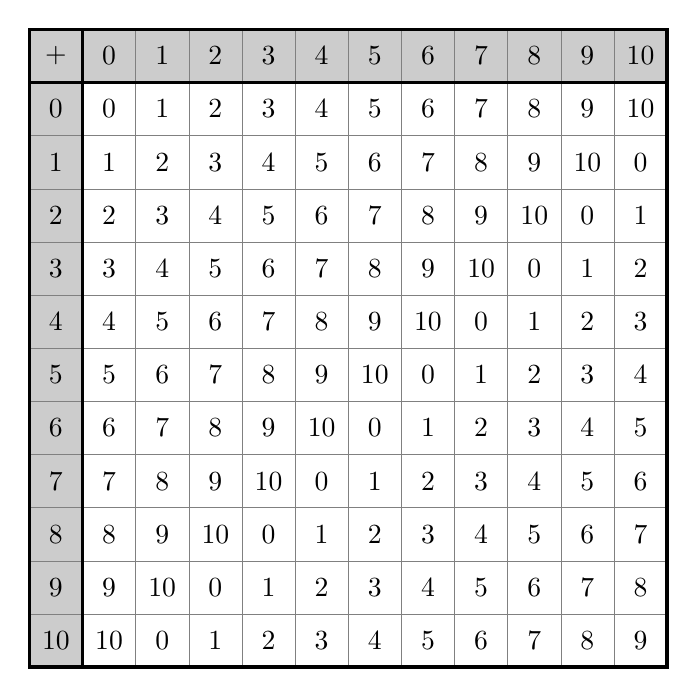
\begin{tikzpicture}[>=latex,thick,scale=0.45]
\fill[color=gray!40] (0,0) rectangle (18,-1.5);
\fill[color=gray!40] (0,0) rectangle (1.5,-18);	
\draw[step = 1.5, gray,very thin] (0,0) grid (18,-18);
\draw[very thick] (0,0) rectangle (18,-18);
\draw[very thick] (0,-1.5) -- (18,-1.5);
\draw[very thick] (1.5,0) -- (1.5,-18);
\node at (0.75,-0.75) {$+$};
\foreach \x in {0,...,10}
	\node at (2.25+\x*1.5,-0.75) {$\x$};
\foreach \y in {0,...,10}
	\node at (0.75,-2.25+\y*-1.5) {$\y$};
% Row 0
\node at ( 2.25,-2.25) {$0$};
\node at ( 3.75,-2.25) {$1$};
\node at ( 5.25,-2.25) {$2$};
\node at ( 6.75,-2.25) {$3$};
\node at ( 8.25,-2.25) {$4$};
\node at ( 9.75,-2.25) {$5$};
\node at (11.25,-2.25) {$6$};
\node at (12.75,-2.25) {$7$};
\node at (14.25,-2.25) {$8$};
\node at (15.75,-2.25) {$9$};
\node at (17.25,-2.25) {$10$};
% Row 1
\node at ( 2.25,-3.75) {$1$};
\node at ( 3.75,-3.75) {$2$};
\node at ( 5.25,-3.75) {$3$};
\node at ( 6.75,-3.75) {$4$};
\node at ( 8.25,-3.75) {$5$};
\node at ( 9.75,-3.75) {$6$};
\node at (11.25,-3.75) {$7$};
\node at (12.75,-3.75) {$8$};
\node at (14.25,-3.75) {$9$};
\node at (15.75,-3.75) {$10$};
\node at (17.25,-3.75) {$0$};
% Row 2
\node at ( 2.25,-5.25) {$2$};
\node at ( 3.75,-5.25) {$3$};
\node at ( 5.25,-5.25) {$4$};
\node at ( 6.75,-5.25) {$5$};
\node at ( 8.25,-5.25) {$6$};
\node at ( 9.75,-5.25) {$7$};
\node at (11.25,-5.25) {$8$};
\node at (12.75,-5.25) {$9$};
\node at (14.25,-5.25) {$10$};
\node at (15.75,-5.25) {$0$};
\node at (17.25,-5.25) {$1$};
% Row 3
\node at ( 2.25,-6.75) {$3$};
\node at ( 3.75,-6.75) {$4$};
\node at ( 5.25,-6.75) {$5$};
\node at ( 6.75,-6.75) {$6$};
\node at ( 8.25,-6.75) {$7$};
\node at ( 9.75,-6.75) {$8$};
\node at (11.25,-6.75) {$9$};
\node at (12.75,-6.75) {$10$};
\node at (14.25,-6.75) {$0$};
\node at (15.75,-6.75) {$1$};
\node at (17.25,-6.75) {$2$};
% Row 4
\node at ( 2.25,-8.25) {$4$};
\node at ( 3.75,-8.25) {$5$};
\node at ( 5.25,-8.25) {$6$};
\node at ( 6.75,-8.25) {$7$};
\node at ( 8.25,-8.25) {$8$};
\node at ( 9.75,-8.25) {$9$};
\node at (11.25,-8.25) {$10$};
\node at (12.75,-8.25) {$0$};
\node at (14.25,-8.25) {$1$};
\node at (15.75,-8.25) {$2$};
\node at (17.25,-8.25) {$3$};
% Row 5
\node at ( 2.25,-9.75) {$5$};
\node at ( 3.75,-9.75) {$6$};
\node at ( 5.25,-9.75) {$7$};
\node at ( 6.75,-9.75) {$8$};
\node at ( 8.25,-9.75) {$9$};
\node at ( 9.75,-9.75) {$10$};
\node at (11.25,-9.75) {$0$};
\node at (12.75,-9.75) {$1$};
\node at (14.25,-9.75) {$2$};
\node at (15.75,-9.75) {$3$};
\node at (17.25,-9.75) {$4$};
% Row 6
\node at ( 2.25,-11.25) {$6$};
\node at ( 3.75,-11.25) {$7$};
\node at ( 5.25,-11.25) {$8$};
\node at ( 6.75,-11.25) {$9$};
\node at ( 8.25,-11.25) {$10$};
\node at ( 9.75,-11.25) {$0$};
\node at (11.25,-11.25) {$1$};
\node at (12.75,-11.25) {$2$};
\node at (14.25,-11.25) {$3$};
\node at (15.75,-11.25) {$4$};
\node at (17.25,-11.25) {$5$};
% Row 7
\node at ( 2.25,-12.75) {$7$};
\node at ( 3.75,-12.75) {$8$};
\node at ( 5.25,-12.75) {$9$};
\node at ( 6.75,-12.75) {$10$};
\node at ( 8.25,-12.75) {$0$};
\node at ( 9.75,-12.75) {$1$};
\node at (11.25,-12.75) {$2$};
\node at (12.75,-12.75) {$3$};
\node at (14.25,-12.75) {$4$};
\node at (15.75,-12.75) {$5$};
\node at (17.25,-12.75) {$6$};
% Row 8
\node at ( 2.25,-14.25) {$8$};
\node at ( 3.75,-14.25) {$9$};
\node at ( 5.25,-14.25) {$10$};
\node at ( 6.75,-14.25) {$0$};
\node at ( 8.25,-14.25) {$1$};
\node at ( 9.75,-14.25) {$2$};
\node at (11.25,-14.25) {$3$};
\node at (12.75,-14.25) {$4$};
\node at (14.25,-14.25) {$5$};
\node at (15.75,-14.25) {$6$};
\node at (17.25,-14.25) {$7$};
% Row 9
\node at ( 2.25,-15.75) {$9$};
\node at ( 3.75,-15.75) {$10$};
\node at ( 5.25,-15.75) {$0$};
\node at ( 6.75,-15.75) {$1$};
\node at ( 8.25,-15.75) {$2$};
\node at ( 9.75,-15.75) {$3$};
\node at (11.25,-15.75) {$4$};
\node at (12.75,-15.75) {$5$};
\node at (14.25,-15.75) {$6$};
\node at (15.75,-15.75) {$7$};
\node at (17.25,-15.75) {$8$};
% Row 10
\node at ( 2.25,-17.25) {$10$};
\node at ( 3.75,-17.25) {$0$};
\node at ( 5.25,-17.25) {$1$};
\node at ( 6.75,-17.25) {$2$};
\node at ( 8.25,-17.25) {$3$};
\node at ( 9.75,-17.25) {$4$};
\node at (11.25,-17.25) {$5$};
\node at (12.75,-17.25) {$6$};
\node at (14.25,-17.25) {$7$};
\node at (15.75,-17.25) {$8$};
\node at (17.25,-17.25) {$9$};
\end{tikzpicture}

\end{center}

%% created by Michael Steiner
%
% Restetabelle von F_11: Multiplikation

% alternatives design
%\begin{figure}
%\begin{center}
%\begin{tabular}{|>{$}c<{$}|>{$}c<{$}>{$}c<{$}>{$}c<{$}>{$}c<{$}>{$}c<{$}>{$}c<{$}>{$}c<{$}>{$}c<{$}>{$}c<{$}>{$}c<{$}>{$}c<{$}|}
%\hline
%\cdot&0&1&2&3&4&5&6&7&8&9&10\\
%\hline
%0&0&0&0&0&0&0&0&0&0&0&0\\
%1&0&1&2&3&4&5&6&7&8&9&10\\
%2&0&2&4&6&8&10&1&3&5&7&9\\
%3&0&3&6&9&1&4&7&10&2&5&8\\
%4&0&4&8&1&5&9&2&6&10&3&7\\
%5&0&5&10&4&9&3&8&2&7&1&6\\
%6&0&6&1&7&2&8&3&9&4&10&5\\
%7&0&7&3&10&6&2&9&5&1&8&4\\
%8&0&8&5&2&10&7&4&1&9&6&3\\
%9&0&9&7&5&3&1&10&8&6&4&2\\
%10&0&10&9&8&7&6&5&4&3&2&1\\
%\hline
%\end{tabular}
%\end{center}
%\end{figure}

\begin{center}
	
	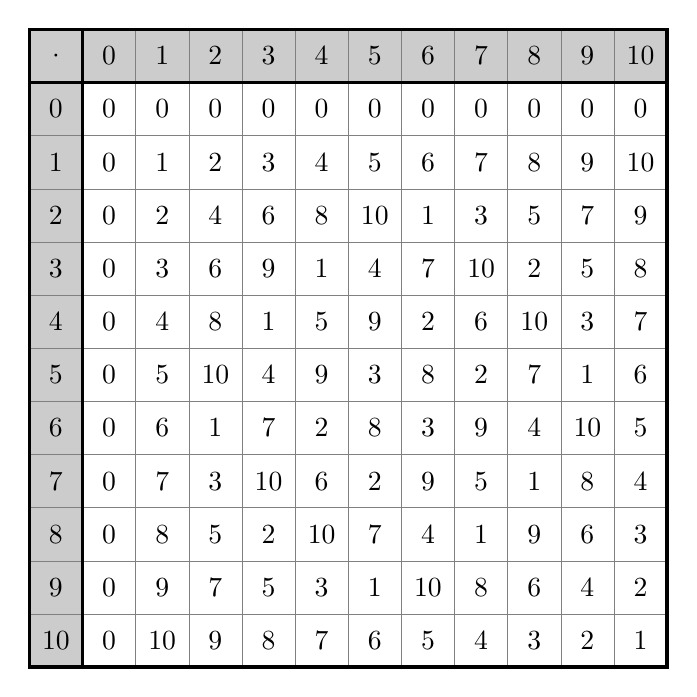
\begin{tikzpicture}[>=latex,thick,scale=0.45]
		\fill[color=gray!40] (0,0) rectangle (18,-1.5);
		\fill[color=gray!40] (0,0) rectangle (1.5,-18);	
		\draw[step = 1.5, gray,very thin] (0,0) grid (18,-18);
		\draw[very thick] (0,0) rectangle (18,-18);
		\draw[very thick] (0,-1.5) -- (18,-1.5);
		\draw[very thick] (1.5,0) -- (1.5,-18);
		\node at (0.75,-0.75) {$\cdot$};
		\foreach \x in {0,...,10}
		\node at (2.25+\x*1.5,-0.75) {$\x$};
		\foreach \y in {0,...,10}
		\node at (0.75,-2.25+\y*-1.5) {$\y$};
		% Row 0
		\node at ( 2.25,-2.25) {$0$};
		\node at ( 3.75,-2.25) {$0$};
		\node at ( 5.25,-2.25) {$0$};
		\node at ( 6.75,-2.25) {$0$};
		\node at ( 8.25,-2.25) {$0$};
		\node at ( 9.75,-2.25) {$0$};
		\node at (11.25,-2.25) {$0$};
		\node at (12.75,-2.25) {$0$};
		\node at (14.25,-2.25) {$0$};
		\node at (15.75,-2.25) {$0$};
		\node at (17.25,-2.25) {$0$};
		% Row 1
		\node at ( 2.25,-3.75) {$0$};
		\node at ( 3.75,-3.75) {$1$};
		\node at ( 5.25,-3.75) {$2$};
		\node at ( 6.75,-3.75) {$3$};
		\node at ( 8.25,-3.75) {$4$};
		\node at ( 9.75,-3.75) {$5$};
		\node at (11.25,-3.75) {$6$};
		\node at (12.75,-3.75) {$7$};
		\node at (14.25,-3.75) {$8$};
		\node at (15.75,-3.75) {$9$};
		\node at (17.25,-3.75) {$10$};
		% Row 2
		\node at ( 2.25,-5.25) {$0$};
		\node at ( 3.75,-5.25) {$2$};
		\node at ( 5.25,-5.25) {$4$};
		\node at ( 6.75,-5.25) {$6$};
		\node at ( 8.25,-5.25) {$8$};
		\node at ( 9.75,-5.25) {$10$};
		\node at (11.25,-5.25) {$1$};
		\node at (12.75,-5.25) {$3$};
		\node at (14.25,-5.25) {$5$};
		\node at (15.75,-5.25) {$7$};
		\node at (17.25,-5.25) {$9$};
		% Row 3
		\node at ( 2.25,-6.75) {$0$};
		\node at ( 3.75,-6.75) {$3$};
		\node at ( 5.25,-6.75) {$6$};
		\node at ( 6.75,-6.75) {$9$};
		\node at ( 8.25,-6.75) {$1$};
		\node at ( 9.75,-6.75) {$4$};
		\node at (11.25,-6.75) {$7$};
		\node at (12.75,-6.75) {$10$};
		\node at (14.25,-6.75) {$2$};
		\node at (15.75,-6.75) {$5$};
		\node at (17.25,-6.75) {$8$};
		% Row 4
		\node at ( 2.25,-8.25) {$0$};
		\node at ( 3.75,-8.25) {$4$};
		\node at ( 5.25,-8.25) {$8$};
		\node at ( 6.75,-8.25) {$1$};
		\node at ( 8.25,-8.25) {$5$};
		\node at ( 9.75,-8.25) {$9$};
		\node at (11.25,-8.25) {$2$};
		\node at (12.75,-8.25) {$6$};
		\node at (14.25,-8.25) {$10$};
		\node at (15.75,-8.25) {$3$};
		\node at (17.25,-8.25) {$7$};
		% Row 5
		\node at ( 2.25,-9.75) {$0$};
		\node at ( 3.75,-9.75) {$5$};
		\node at ( 5.25,-9.75) {$10$};
		\node at ( 6.75,-9.75) {$4$};
		\node at ( 8.25,-9.75) {$9$};
		\node at ( 9.75,-9.75) {$3$};
		\node at (11.25,-9.75) {$8$};
		\node at (12.75,-9.75) {$2$};
		\node at (14.25,-9.75) {$7$};
		\node at (15.75,-9.75) {$1$};
		\node at (17.25,-9.75) {$6$};
		% Row 6
		\node at ( 2.25,-11.25) {$0$};
		\node at ( 3.75,-11.25) {$6$};
		\node at ( 5.25,-11.25) {$1$};
		\node at ( 6.75,-11.25) {$7$};
		\node at ( 8.25,-11.25) {$2$};
		\node at ( 9.75,-11.25) {$8$};
		\node at (11.25,-11.25) {$3$};
		\node at (12.75,-11.25) {$9$};
		\node at (14.25,-11.25) {$4$};
		\node at (15.75,-11.25) {$10$};
		\node at (17.25,-11.25) {$5$};
		% Row 7
		\node at ( 2.25,-12.75) {$0$};
		\node at ( 3.75,-12.75) {$7$};
		\node at ( 5.25,-12.75) {$3$};
		\node at ( 6.75,-12.75) {$10$};
		\node at ( 8.25,-12.75) {$6$};
		\node at ( 9.75,-12.75) {$2$};
		\node at (11.25,-12.75) {$9$};
		\node at (12.75,-12.75) {$5$};
		\node at (14.25,-12.75) {$1$};
		\node at (15.75,-12.75) {$8$};
		\node at (17.25,-12.75) {$4$};
		% Row 8
		\node at ( 2.25,-14.25) {$0$};
		\node at ( 3.75,-14.25) {$8$};
		\node at ( 5.25,-14.25) {$5$};
		\node at ( 6.75,-14.25) {$2$};
		\node at ( 8.25,-14.25) {$10$};
		\node at ( 9.75,-14.25) {$7$};
		\node at (11.25,-14.25) {$4$};
		\node at (12.75,-14.25) {$1$};
		\node at (14.25,-14.25) {$9$};
		\node at (15.75,-14.25) {$6$};
		\node at (17.25,-14.25) {$3$};
		% Row 9
		\node at ( 2.25,-15.75) {$0$};
		\node at ( 3.75,-15.75) {$9$};
		\node at ( 5.25,-15.75) {$7$};
		\node at ( 6.75,-15.75) {$5$};
		\node at ( 8.25,-15.75) {$3$};
		\node at ( 9.75,-15.75) {$1$};
		\node at (11.25,-15.75) {$10$};
		\node at (12.75,-15.75) {$8$};
		\node at (14.25,-15.75) {$6$};
		\node at (15.75,-15.75) {$4$};
		\node at (17.25,-15.75) {$2$};
		% Row 10
		\node at ( 2.25,-17.25) {$0$};
		\node at ( 3.75,-17.25) {$10$};
		\node at ( 5.25,-17.25) {$9$};
		\node at ( 6.75,-17.25) {$8$};
		\node at ( 8.25,-17.25) {$7$};
		\node at ( 9.75,-17.25) {$6$};
		\node at (11.25,-17.25) {$5$};
		\node at (12.75,-17.25) {$4$};
		\node at (14.25,-17.25) {$3$};
		\node at (15.75,-17.25) {$2$};
		\node at (17.25,-17.25) {$1$};
	\end{tikzpicture}
	
\end{center}

Die grösse des endlichen Körpers legt auch fest, wie gross unsere Nachricht $n$ bestehend aus Nutzdatenteil und Fehlerkorrekturteil sein kann und beträgt in unserem Beispiel
\[
n = q - 1 = 10 \text{ Zahlen}.
\]

Im nächsten Schritt bestimmen wir, wie viele Fehler $t$ maximal während der Übertragung auftreten dürfen, damit wir sie noch korrigieren können.
Unser Beispielcode sollte in der Lage sein
\[
t = 2
\]
Fehlerstellen korrigieren zu können.

Die Grösse des Nutzdatenteils hängt von der Grösse der Nachricht sowie der Anzahl der Fehlerkorrekturstellen. Je robuster der Code sein muss, desto weniger Platz für Nutzdaten $k$ bleibt in der Nachricht übrig.
Bei maximal 2 Fehler können wir noch
\[
k = n - 2t = 6\text{ Zahlen}
\]
übertragen. 

Zusammenfassend haben wir einen Codeblock mit der Länge von 10 Zahlen definiert, der 6 Zahlen als Nutzlast beinhaltet und in der Lage ist aus 2 fehlerhafte Stellen im Block die ursprünglichen Nutzdaten rekonstruieren kann. Zudem werden wir im weiteren feststellen, dass dieser Code maximal 4 Fehlerstellen erkennen, diese aber nicht rekonstruieren kann.

Wir legen nun die Nachricht
\[
m = [0,0,0,0,4,7,2,5,8,1]
\]
fest, die wir gerne an einen Empfänger übertragen möchten, wobei die vorderen vier Nullstellen für die Fehlerkorrektur zuständig sind.
Die Nachricht können wir auch als Polynom 
\[
m(X) = 4X^5 + 7X^4 + 2X^3 + 5X^2 + 8X + 1
\] 
darstellen.

\subsection{Der Ansatz der diskreten Fouriertransformation
	\label{reedsolomon:subsection:diskFT}}

In einem vorherigen Kapitel (???) haben wir schon einmal die diskrete Fouriertransformation zum Codieren einer Nachricht verwendet. In den endlichen Körpern wird dies jedoch nicht gelingen, da die Eulerische Zahl $\mathrm{e}$ in $\mathbb{F}_{11}$ nicht existiert. 
Wir suchen also eine Zahl $a^i$, die in endlichen Körpern existiert und den gesamten Zahlenbereich von $\mathbb{F}_{11}$ abdecken kann.
Dazu schreiben wir
\[
\mathbb{F}_{11} = \{0,1,2,3,4,5,6,7,8,9,10\}
\]
um in 
\[
\mathbb{Z}_{11}\setminus\{0\} = \{a^0, a^1, a^2, a^3, a^4, a^5, a^6, a^7, a^8, a^9\}.
\]

Wenn wir alle möglichen Werte für $a$ einsetzen, also

%\begin{align}
%a = 0 : \qquad \mathbb{Z}_{11}\setminus\{0\} = \{0, 0, 0, 0, 0, 0, 0, 0, 0, 0\} \\
%a = 1 : \qquad \mathbb{Z}_{11}\setminus\{0\} = \{1, 1, 1, 1, 1, 1, 1, 1, 1, 1\} \\
%a = 2 : \qquad \mathbb{Z}_{11}\setminus\{0\} = \{1, 2, 4, 8, 5, 10, 9, 7, 3, 6\} \\
%a = 3 : \qquad \mathbb{Z}_{11}\setminus\{0\} = \{1, 3, 9, 5, 4, 1, 3, 9, 5, 4\} \\
%a = 4 : \qquad \mathbb{Z}_{11}\setminus\{0\} = \{1, 4, 5, 9, 3, 1, 4, 5, 9, 3\} \\
%a = 5 : \qquad \mathbb{Z}_{11}\setminus\{0\} = \{1, 5, 3, 4, 9, 1, 5, 3, 4, 9\} \\
%a = 6 : \qquad \mathbb{Z}_{11}\setminus\{0\} = \{1, 6, 3, 7, 9, 10, 5, 8, 4, 2\} \\
%a = 7 : \qquad \mathbb{Z}_{11}\setminus\{0\} = \{1, 7, 5, 2, 3, 10, 4, 6, 9, 8\} \\
%a = 8 : \qquad \mathbb{Z}_{11}\setminus\{0\} = \{1, 8, 9, 6, 4, 10, 3, 2, 5, 7\} \\
%a = 9 : \qquad \mathbb{Z}_{11}\setminus\{0\} = \{1, 9, 4, 3, 5, 1, 9, 4, 3, 5\} \\
%a = 10 : \qquad \mathbb{Z}_{11}\setminus\{0\} = \{1, 10, 1, 10, 1, 10, 1, 10, 1, 10\}
%\end{align}

\begin{center}
\begin{tabular}{c r c l}
%$a = 0 :$& $\qquad \mathbb{Z}_{11}\setminus\{0\}$ &$=$& $\{0, 0, 0, 0, 0, 0, 0, 0, 0, 0\}$ \\
$a = 1 :$& $\qquad \mathbb{Z}_{11}\setminus\{0\}$ &$=$& $\{1, 1, 1, 1, 1, 1, 1, 1, 1, 1\}$ \\
$a = 2 :$& $\qquad \mathbb{Z}_{11}\setminus\{0\}$ &$=$& $\{1, 2, 4, 8, 5, 10, 9, 7, 3, 6\}$ \\
$a = 3 :$& $\qquad \mathbb{Z}_{11}\setminus\{0\}$ &$=$& $\{1, 3, 9, 5, 4, 1, 3, 9, 5, 4\}$ \\
$a = 4 :$& $\qquad \mathbb{Z}_{11}\setminus\{0\}$ &$=$& $\{1, 4, 5, 9, 3, 1, 4, 5, 9, 3\}$ \\
$a = 5 :$& $\qquad \mathbb{Z}_{11}\setminus\{0\}$ &$=$& $\{1, 5, 3, 4, 9, 1, 5, 3, 4, 9\}$ \\
$a = 6 :$& $\qquad \mathbb{Z}_{11}\setminus\{0\}$ &$=$& $\{1, 6, 3, 7, 9, 10, 5, 8, 4, 2\}$ \\
$a = 7 :$& $\qquad \mathbb{Z}_{11}\setminus\{0\}$ &$=$& $\{1, 7, 5, 2, 3, 10, 4, 6, 9, 8\}$ \\
$a = 8 :$& $\qquad \mathbb{Z}_{11}\setminus\{0\}$ &$=$& $\{1, 8, 9, 6, 4, 10, 3, 2, 5, 7\}$ \\
$a = 9 :$& $\qquad \mathbb{Z}_{11}\setminus\{0\}$ &$=$& $\{1, 9, 4, 3, 5, 1, 9, 4, 3, 5\}$ \\
$a = 10 :$& $\qquad \mathbb{Z}_{11}\setminus\{0\}$ &$=$& $\{1, 10, 1, 10, 1, 10, 1, 10, 1, 10\}$	
\end{tabular}
\end{center}

so fällt uns auf, dass die Zahlen $2,6,7,8$ tatsächlich den gesamten Zahlenraum von $\mathbb{F}_{11}$ abbilden. Solche Zahlen werden \em Primitive Einheitswurzel \em genannt. 
Für das Beispiel wählen wir die Zahl $a^i = 8$.
Damit wir unsere Nachricht codieren können, müssen wir $8^i$ in $m(X)$ einsetzen.

\begin{center}
	\begin{tabular}{c}
		$m(8^0) = 4 \cdot 1 + 7 \cdot 1 + 2 \cdot 1 + 5 \cdot 1 + 8 \cdot 1 + 1 = 5$ \\
		$m(8^1) = 4 \cdot 8 + 7 \cdot 8 + 2 \cdot 8 + 5 \cdot 8 + 8 \cdot 8 + 1 = 3$ \\
		\vdots
	\end{tabular}
\end{center}

Für eine elegantere Formulierung stellen wir das ganze als Matrix dar, wobei $m$ unser Nachrichtenvektor, $A$ die Transformationsmatrix und $v$ unser Übertragungsvektor ist. 
	
\[
v = A \cdot m \qquad \Rightarrow \qquad v = \begin{pmatrix}
	8^0&    8^0&    8^0&    8^0&    8^0&    8^0&    8^0&    8^0&    8^0&    8^0\\
	8^0&	8^1&	8^2&	8^3&	8^4&	8^5&	8^6&	8^7&    8^8&	8^9\\
	8^0&	8^2&	8^4&	8^6&	8^8& 8^{10}& 8^{12}& 8^{14}& 8^{16}& 8^{18}\\
	8^0&	8^3&	8^6&	8^9& 8^{12}& 8^{15}& 8^{18}& 8^{21}& 8^{24}& 8^{27}\\
	8^0&	8^4&	8^8& 8^{12}& 8^{16}& 8^{20}& 8^{24}& 8^{28}& 8^{32}& 8^{36}\\
	8^0&	8^5& 8^{10}& 8^{15}& 8^{20}& 8^{25}& 8^{30}& 8^{35}& 8^{40}& 8^{45}\\
	8^0&	8^6& 8^{12}& 8^{18}& 8^{24}& 8^{30}& 8^{36}& 8^{42}& 8^{48}& 8^{54}\\
	8^0&	8^7& 8^{14}& 8^{21}& 8^{28}& 8^{35}& 8^{42}& 8^{49}& 8^{56}& 8^{63}\\
	8^0&	8^8& 8^{16}& 8^{24}& 8^{32}& 8^{40}& 8^{48}& 8^{56}& 8^{64}& 8^{72}\\
	8^0&	8^9& 8^{18}& 8^{27}& 8^{36}& 8^{45}& 8^{54}& 8^{63}& 8^{72}& 8^{81}\\
\end{pmatrix}
\cdot
\begin{pmatrix}
	1 \\ 8 \\ 5 \\ 2 \\ 7 \\ 4 \\ 0 \\ 0 \\ 0 \\ 0 \\
\end{pmatrix}
\]

Somit bekommen wir für unseren Übertragungsvektor
\[
v = [5,3,6,5,2,10,2,7,10,4],
\]
den wir jetzt über einen beliebigen Nachrichtenkanal versenden können.

\textbf{NOTES}

warum wird 0 weggelassen?

%
% teil3.tex -- Beispiel-File für Teil 3
%
% (c) 2020 Prof Dr Andreas Müller, Hochschule Rapperswil
%
\section{Decodierung ohne Fehler
\label{reedsolomon:section:decohnefehler}}
\rhead{fehlerlose rekonstruktion}
Im ersten Teil zur Decodierung des Übertragungsvektor betrachten wir den Übertragungskanal als fehlerfrei.
Wir erhalten also unseren Übertragungsvektor
\[
v = [5,3,6,5,2,10,2,7,10,4].
\]

Gesucht ist nun einen Weg, mit dem wir auf unseren Nachrichtenvektor zurückrechnen können.
Ein banaler Ansatz ist das Invertieren der Glechung
\[
v = A \cdot m \qquad \Rightarrow \qquad m = A^{-1} \cdot v.
\]

Nur stellt sich dann die Frage, wie wir auf die Inverse der Matix $A$ kommen.
Dazu können wir wiederum den Ansatz der Fouriertransformation uns zur Hilfe nehmen,
jedoch betrachten wir jetzt deren Inverse.
Definiert ist sie als
\[
F(\omega) = \int_{-\infty}^{\infty} f(t) \mathrm{e}^{-j\omega t} dt \qquad \Rightarrow \qquad \mathfrak{F}^{-1}(F(\omega)) = f(t) = \frac{1}{2 \pi} \int_{-\infty}^{\infty} F(\omega) \mathrm{e}^{j \omega t} d\omega.
\]

In unserem Fall suchen wir also eine inverse für die Primitive Einheitswurzel $a$, also
\[
8^1 \qquad \Rightarrow \qquad 8^{-1}.
\]

Im Abschnitt \textcolor{red}{4.1} haben wir den euklidischen Algorithmus kennengelernt, den wir auf unseren Fall anwenden können.

\subsection{Der Euklidische Algorithmus
\label{reedsolomon:subsection:eukAlgo}}

Die Funktionsweise des euklidischen Algorithmus ist im Kapitel \textcolor{red}{4.1} ausführlich beschrieben.
Für unsere Anwendung wählen wir die Parameter $a_i = 8$ und $b_i = 11$.
Daraus erhalten wir 

\begin{center}

\begin{tabular}{| c | c c | c | r r |}
	\hline
	$k$ & $a_i$ & $b_i$ & $q_i$ & $c_i$ & $d_i$\\
	\hline 
	& & & & $1$& $0$\\
	$0$& $8$& $11$& $0$& $0$& $1$\\
	$1$& $11$& $8$& $1$& $1$& $0$\\
	$2$& $8$& $3$& $2$& $-1$& $1$\\
	$3$& $3$& $2$& $1$& $3$& $-2$\\
	$4$& $2$& $1$& $2$& \textcolor{blue}{$-4$}& \textcolor{red}{$3$}\\
	$5$& $1$& $0$& & $11$& $-8$\\
	\hline
\end{tabular}

\end{center}
\begin{center}

\begin{tabular}{rcl}
	$\textcolor{blue}{-4} \cdot 8 + \textcolor{red}{3} \cdot 11$ &$=$& $1$\\
	$7 \cdot 8 + 3 \cdot 11$ &$=$& $1$\\
	$8^{-1}$ &$=$& $7$
	
\end{tabular}

\end{center}

als Inverse der Primitiven Einheitswurzel.

Nun haben wir fast alles für die Rücktransformation beisammen. Wie auch bei der Inversen Fouriertransformation haben wir nun einen Vorfaktor
\[
m = \textcolor{red}{s} \cdot A^{-1} \cdot v
\]
den wir noch bestimmen müssen. 
Glücklicherweise lässt der sich analog wie bei der Inversen Fouriertransformation bestimmen und beträgt
\[
s = \frac{1}{10}.
\]
Da $\frac{1}{10} = 10^{-1}$ entspricht können wir $s$ ebenfalls mit dem euklidischen Algorithmus bestimmen und stellen fest, dass $10^{-1} = 10$ ergibt.
Somit lässt sich den Nachrichtenvektor einfach bestimmen mit
\[
m = 10 \cdot A^{-1} \cdot v \qquad \Rightarrow \qquad m = 10 \cdot \begin{pmatrix}
	7^0&    7^0&    7^0&    7^0&    7^0&    7^0&    7^0&    7^0&    7^0&    7^0\\
	7^0&	7^1&	7^2&	7^3&	7^4&	7^5&	7^6&	7^7&    7^8&	7^9\\
	7^0&	7^2&	7^4&	7^6&	7^8& 7^{10}& 7^{12}& 7^{14}& 7^{16}& 7^{18}\\
	7^0&	7^3&	7^6&	7^9& 7^{12}& 7^{15}& 7^{18}& 7^{21}& 7^{24}& 7^{27}\\
	7^0&	7^4&	7^8& 7^{12}& 7^{16}& 7^{20}& 7^{24}& 7^{28}& 7^{32}& 7^{36}\\
	7^0&	7^5& 7^{10}& 7^{15}& 7^{20}& 7^{25}& 7^{30}& 7^{35}& 7^{40}& 7^{45}\\
	7^0&	7^6& 7^{12}& 7^{18}& 7^{24}& 7^{30}& 7^{36}& 7^{42}& 7^{48}& 7^{54}\\
	7^0&	7^7& 7^{14}& 7^{21}& 7^{28}& 7^{35}& 7^{42}& 7^{49}& 7^{56}& 7^{63}\\
	7^0&	7^8& 7^{16}& 7^{24}& 7^{32}& 7^{40}& 7^{48}& 7^{56}& 7^{64}& 7^{72}\\
	7^0&	7^9& 7^{18}& 7^{27}& 7^{36}& 7^{45}& 7^{54}& 7^{63}& 7^{72}& 7^{81}\\
\end{pmatrix}
\cdot
\begin{pmatrix}
	5 \\ 3 \\ 6 \\ 5 \\ 2 \\ 10 \\ 2 \\ 7 \\ 10 \\ 4 \\
\end{pmatrix}
\]
und wir erhalten
\[
m = [0,0,0,0,4,7,2,5,8,1]
\]
als unsere Nachricht zurück.
%
% teil3.tex -- Beispiel-File für Teil 3
%
% (c) 2020 Prof Dr Andreas Müller, Hochschule Rapperswil
%
\section{Decodierung mit Fehler
\label{reedsolomon:section:decmitfehler}}
\rhead{fehlerhafte rekonstruktion}
Im zweiten Teil zur Decodierung betrachten wir den Fall, dass unser Übertragungskanal nicht fehlerfrei ist.
Wir legen daher den Fehlervektor
\[
u = [0, 0, 0, 3, 0, 0, 0, 0, 2, 0]
\]
fest, den wir zu unserem Übertragungsvektor als Fehler dazu addieren und somit

\begin{center}

\begin{tabular}{c | c r }
	$v$ & & $[5,3,6,5,2,10,2,7,10,4]$\\
	$u$ & $+$ & $[0,0,0,3,0,0,0,0,2,0]$\\
	\hline
	$w$ & & $[5,3,6,8,2,10,2,7,1,4]$\\
\end{tabular}

% alternative design
%\begin{tabular}{c | c cccccccccccc }
%	$v$ & & $[$&$5,$&$3,$&$6,$&$5,$&$2,$&$10,$&$2,$&$7,$&$10,$&$4$&$]$\\
%	$u$ & $+$ & $[$&$0,$&$0,$&$0,$&$3,$&$0,$&$0,$&$0,$&$0,$&$2,$&$0$&$]$\\
%	\hline
%	$w$ & & $[$&$5,$&$3,$&$6,$&$8,$&$2,$&$10,$&$2,$&$7,$&$1,$&$4$&$]$\\
%\end{tabular}

\end{center}
als Übertragungsvektor auf der Empfängerseite erhalten. 

Wenn wir den Übertragungsvektor jetzt Rücktransformieren wie im vorherigen Kapitel erhalten wir
\[
r = [\underbrace{5,7,4,10,}_{Fehlerinfo}5,4,5,7,6,7].
\]
Im Vergleich zum vorherigen Kapitel sind die Fehlerkorrekturstellen jetzt $\neq 0$, was bedeutet, dass wir diesen Übertragungsvektor fehlerhaft empfangen haben und sich die Nachricht jetzt nicht mehr so einfach decodieren lässt.

% warum wir die fehler suchen
Da Reed-Solomon-Codes in der Lage sind, eine Nachricht aus weniger Stellen zu rekonstruieren als wir ursprünglich haben, so müssen wir nur die Fehlerhaften Stellen finden und eliminieren, damit wir unsere Nutzdaten rekonstruieren können.
Damit stellt sich die Frage, wie wir die Fehlerstellen $e$ finden.
Dafür wählen wir einen Primitiven Ansatz mit
\begin{align}
	m(X) & = 4X^5 + 7X^4 + 2X^3 + 5X^2 + 8X + 1 \\
	r(X) & = 5X^9 + 7X^8 + 4X^7 + 10X^6 + 5X^5 + 4X^4 + 5X^3 + 7X^2 + 6X + 7 \\
	e(X) & = r(X) - m(X).
\end{align}
Setzen wir jetzt unsere Einheitswurzel für $X$ ein, so erhalten wir
\begin{center}
\begin{tabular}{c c c c c c c c c c c}
	\hline
	$i$& $0$& $1$& $2$& $3$& $4$& $5$& $6$& $7$& $8$& $9$\\
	\hline
	$r(a^{i})$& $5$& $3$& $6$& $8$& $2$& $10$& $2$& $7$& $1$& $4$\\
	$m(a^{i})$& $5$& $3$& $6$& $5$& $2$& $10$& $2$& $7$& $10$& $4$\\
	$e(a^{i})$& $0$& $0$& $0$& $3$& $0$& $0$& $0$& $0$& $2$& $0$\\
	\hline
\end{tabular}
\end{center}
und damit die Information, dass an allen Stellen, die nicht Null sind, Fehler enthalten.
Um jetzt alle nicht Nullstellen zu finden, wenden wir den Satz von Fermat an. 

\subsection{Der Satz von Fermat
\label{reedsolomon:subsection:fermat}}
Der Satz von Fermat besagt, dass für
\[
f(X) = X^{q-1} -1 = 0
\] 
gilt, egal was wir für $q$ einsetzen.

Für unser Beispiel erhalten wir
\[
f(X) = X^{10}-1 = 0 \qquad \text{für } X = \{1,2,3,4,5,6,7,8,9,10\}
\]
und können $f(X)$ auch umschreiben in
\[
f(X) = (X-a^0)(X-a^1)(X-a^2)(X-a^3)(X-a^4)(X-a^5)(X-a^6)(X-a^7)(X-a^8)(X-a^9).
\]
Zur Überprüfung können wir unsere Einheitswurzel in $a$ einsetzen und werden sehen, dass wir für $f(X) = 0$ erhalten werden.
Nach der gleichen Überlegung können wir jetzt auch $e(X)$ darstellen als
\[
e(X) = (X-a^0)(X-a^1)(X-a^2) \qquad \qquad (X-a^4)(X-a^5)(X-a^6)(X-a^7) \qquad \qquad (X-a^9) \cdot p(x),
\]
wobei $p(X)$ das Restpolynom ist und die Fehlerstellen beinhaltet.
Wenn wir jetzt den grössten gemeinsamen Teiler von $f(X)$ und $e(X)$ berechnen, so erhalten wir mit
\[
\operatorname{ggT}(f(X),e(X)) = (X-a^0)(X-a^1)(X-a^2) \qquad \qquad (X-a^4)(X-a^5)(X-a^6)(X-a^7) \qquad \qquad (X-a^9)
\]
eine Liste von Nullstellen, an denen es keine Fehler gegeben hat.
Da wir uns jedoch für eine Liste mit Nullstellen interessieren, an denen es Fehler gegeben hat berechnen wir stattdessen das kgV von $f(X)$ und $e(X)$ als
\[
\operatorname{kgV}(f(X),e(X)) = (X-a^0)(X-a^1)(X-a^2)(X-a^3)(X-a^4)(X-a^5)(X-a^6)(X-a^7)(X-a^8)(X-a^9) \cdot q(X).
\]
Wir können das Resultat noch zerlegen in
\[
\operatorname{kgV}(f(X),e(X)) = d(X) \cdot e(X).
\]
Somit muss $d(X)$ eine Liste von Nullstellen enthalten an denen es Fehler gegeben hat.
\[
d(X) = (X-a^3)(X-a^8)
\]


und ist damit unser gesuchtes Lokatorpolynom.

Das einzige Problem was jetzt noch bleibt ist, dass wir $e(X)$ berechnet haben aus
\[
e(X) = r(X) - m(X),
\]
wobei $m(X)$ auf der Empfängerseite unbekannt ist.
Es sieht danach aus, das wir diesen Lösungsansatz nicht verwenden können, da uns ein entscheidender Teil fehlt.
Bei einer näheren Betrachtung von $m(X)$ fällt uns aber auf, dass wir doch etwas über $m(X)$ wissen.
Wir kennen nämlich die ersten vier Stellen, da diese für die Fehlerkorrektur zuständig sind und daher Null sein müssen.
\[
m = [0,0,0,0,?,?,?,?,?,?]
\]
An genau diesen Stellen liegt auch die Information, wo unsere Fehlerstellen liegen, was uns ermöglicht, den Teil von $e(X)$ zu berechnen, der uns auch interessiert.

Wir können $e(X)$ also bestimmen als
\[
e(X) = 5X^9 + 7X^8 + 4X^7 + 10X^6 + p(X)
\]
wobei $p(X)$ wiederum ein unbekanntes Restpolynom ist und
\[
f(X) = X^{10} - 1 = X^{10} + 10
\]
ist können wir so in einer ersten Instanz den grössten gemeinsamen Teiler von $f(X)$ und $e(X)$ berechnen.
Dafür nehmen wir uns wiederum den Euklidischen Algorithmus zur Hilfe und berechnen so

\[
\arraycolsep=1.4pt
\begin{array}{rcrcrcrcccrcrcrcrcrcrcrcrcr}
	X^{10}& & & & & & &+& 10& & & & &:&5X^9&+&7X^8&+& 4X^7&+&10X^6&+&p(X)&=&9X&+&5\\
	X^{10}&+& 8X^9&+& 3X^8&+&2X^7&+& p(X)& &  & & & &   & & & & & &   & &  & & \\ \cline{1-9}
	&& 3X^9&+& 8X^8&+& 9X^7&+& p(X)& &   & & & & & &   & &  & & \\
	&& 3X^9&+& 2X^8&+& 9X^7&+& p(X)& &   & & & & & &   & &  & & \\ \cline{3-9}
	& &    & &6X^8&+&0X^7&+&p(X)& &   & & & & & &   & &  & & \\
\end{array}
\]

\[
\arraycolsep=1.4pt
\begin{array}{rcrcrcrcccrcrcrcrcrcrcrcrcr}
	5X^9&+& 7X^8&+& 4X^7&+& 10X^6&+& p(X)& & & & &:&6X^8&+&0X^7& & & & & & &=&10X&+&3\\
	5X^9&+& 0X^8&+& p(X)& & & & & &  & & & &   & & & & & &   & &  & & \\ \cline{1-5}
	&& 7X^8&+& p(X)& & & & & &   & & & & & &   & &  & & \\
\end{array}
\]
und erhalten
\[
\operatorname{ggT}(f(X),e(X)) = 6X^8
\]
Mit den Resultaten, die wir vom Rechenweg des grössten gemeinsamen Teiler erhalten haben können wir jetzt auch das kleinste Gemeinsame Vielfache berechnen. Eine detailliertere Vorgehensweise findet man in Kapitel ???. 

Aus diesem erweiterten Euklidischen Algorithmus erhalten wir 
\begin{center}
	
	\begin{tabular}{| c | c | c c |}
		\hline
		$k$ &  $q_i$ & $e_i$ & $f_i$\\
		\hline 
		& & $0$& $1$\\
		$0$& $9X + 5$& $1$& $0$\\
		$1$& $10X + 3$& $9X+5$& $1$\\
		$2$& & \textcolor{blue}{$2X^2 + 0X + 5$}& $10X + 3$\\
		\hline
	\end{tabular}	
	
\end{center}
und erhalten auf diesem Weg den Faktor
\[
d(X) = 2X^2 + 5,
\]
den wir in 
\[
d(X) = 2(X-5)(X-6)
\]
zerlegen können.
Da die unbekannten Stellen im Lokatorpolynom
\[
d(X) = (X-a^i)(X-a^i)
\]
sind, müssen wir nur noch $i$ berechnen als
\begin{center}
	$a^i = 5 \qquad \Rightarrow \qquad i = 3$
	
	$a^i = 6 \qquad \Rightarrow \qquad i = 8$.
\end{center}

Somit erhalten wir schliesslich
\[
d(X) = (X-a^3)(X-a^8)
\]
als unser Lokatorpolynom mit den Fehlerhaften Stellen.
%
% rekonstruktion.tex
% Autor: Michael Steiner
%
% (c) 2020 Prof Dr Andreas Müller, Hochschule Rapperswil
%
\section{Nachricht Rekonstruieren
\label{reedsolomon:section:rekonstruktion}}
\rhead{Rekonstruktion}
Im letzten Kapitel haben wir eine Möglichkeit gefunden, wie wir die fehlerhaften Stellen lokalisieren können.
Mit diesen Stellen soll es uns nun möglich sein, aus dem fehlerhaften empfangenen Nachrichtenvektor wieder unsere Nachricht zu rekonstruieren.
Das Lokatorpolynom
\[
l(X) = (X - a^3)(X-a^8)
\]
markiert dabei diese fehlerhaften Stellen im Übertragungsvektor
\[
w = [5,3,6,8,2,10,2,7,1,4].
\]
Als Ausgangslage verwenden wir die Matrix, mit der wir den Nachrichtenvektor ursprünglich codiert haben.
Unser Ziel ist es wie auch schon im Abschnitt \ref{reedsolomon:section:decohnefehler} eine Möglichkeit zu finden, wie wir den Übertragungsvektor decodieren können. 
Aufgrund der Fehlerstellen müssen wir aber davon ausgehen, das wir nicht mehr den gleichen Weg verfolgen können wie wir im Abschnitt \ref{reedsolomon:section:decohnefehler} angewendet haben.

Wir stellen also die Matrix auf und markieren gleichzeitig die Fehlerstellen.
\[
\textcolor{gray}{
	\begin{pmatrix}
		a^0 \\ a^1 \\ a^2 \\ \textcolor{red}{a^3} \\ a^4 \\ a^5 \\ a^6 \\ a^7 \\ \textcolor{red}{a^8} \\ a^9 \\
\end{pmatrix}}
\begin{pmatrix}
	5 \\ 3 \\ 6 \\ \textcolor{red}{8} \\ 2 \\ 10 \\ 2 \\ 7 \\ \textcolor{red}{1} \\ 4 \\
\end{pmatrix}
=
\begin{pmatrix}
	8^0&    8^0&    8^0&    8^0&    8^0&    8^0&    8^0&    8^0&    8^0&    8^0\\
	8^0&	8^1&	8^2&	8^3&	8^4&	8^5&	8^6&	8^7&    8^8&	8^9\\
	8^0&	8^2&	8^4&	8^6&	8^8& 8^{10}& 8^{12}& 8^{14}& 8^{16}& 8^{18}\\
	\textcolor{red}{8^0}&	\textcolor{red}{8^3}&	\textcolor{red}{8^6}&	\textcolor{red}{8^9}& \textcolor{red}{8^{12}}& \textcolor{red}{8^{15}}& \textcolor{red}{8^{18}}& \textcolor{red}{8^{21}}& \textcolor{red}{8^{24}}& \textcolor{red}{8^{27}}\\
	8^0&	8^4&	8^8& 8^{12}& 8^{16}& 8^{20}& 8^{24}& 8^{28}& 8^{32}& 8^{36}\\
	8^0&	8^5& 8^{10}& 8^{15}& 8^{20}& 8^{25}& 8^{30}& 8^{35}& 8^{40}& 8^{45}\\
	8^0&	8^6& 8^{12}& 8^{18}& 8^{24}& 8^{30}& 8^{36}& 8^{42}& 8^{48}& 8^{54}\\
	8^0&	8^7& 8^{14}& 8^{21}& 8^{28}& 8^{35}& 8^{42}& 8^{49}& 8^{56}& 8^{63}\\
	\textcolor{red}{8^0}&	\textcolor{red}{8^8}& \textcolor{red}{8^{16}}& \textcolor{red}{8^{24}}& \textcolor{red}{8^{32}}& \textcolor{red}{8^{40}}& \textcolor{red}{8^{48}}& \textcolor{red}{8^{56}}& \textcolor{red}{8^{64}}& \textcolor{red}{8^{72}}\\
	8^0&	8^9& 8^{18}& 8^{27}& 8^{36}& 8^{45}& 8^{54}& 8^{63}& 8^{72}& 8^{81}\\
\end{pmatrix}
\cdot
\begin{pmatrix}
	m_0 \\ m_1 \\ m_2 \\ m_3 \\ m_4 \\ m_5 \\ m_6 \\ m_7 \\ m_8 \\ m_9 \\
\end{pmatrix}
\]
Die rot markierten Stellen im Übertragungsvektor enthalten Fehler und bringt uns daher kein weiterer Nutzen. 
Aus diesem Grund werden diese Stellen aus dem Vektor entfernt, was wir hier ohne Probleme machen können, da dieser Code ja über Fehlerkorrekturstellen verfügt, deren Aufgabe es ist, eine bestimmte Anzahl an Fehler kompensieren zu können.
Die dazugehörigen Zeilen in der Matrix werden ebenfalls entfernt, da die Matrix gleich viele Zeilen wie im Übertragungsvektor aufweisen muss, damit man ihn decodieren kann.

Daraus resultiert
\[
\begin{pmatrix}
	5 \\ 3 \\ 6 \\ 2 \\ 10 \\ 2 \\ 7 \\ 4 \\
\end{pmatrix}
=
\begin{pmatrix}
	8^0&    8^0&    8^0&    8^0&    8^0&    8^0&    8^0&    8^0&    8^0&    8^0\\
	8^0&	8^1&	8^2&	8^3&	8^4&	8^5&	8^6&	8^7&    8^8&    8^9\\
	8^0&	8^2&	8^4&	8^6&	8^8& 8^{10}& 8^{12}& 8^{14}& 8^{16}& 8^{18}\\
	8^0&	8^4&	8^8& 8^{12}& 8^{16}& 8^{20}& 8^{24}& 8^{28}& 8^{32}& 8^{36}\\
	8^0&	8^5& 8^{10}& 8^{15}& 8^{20}& 8^{25}& 8^{30}& 8^{35}& 8^{40}& 8^{45}\\
	8^0&	8^6& 8^{12}& 8^{18}& 8^{24}& 8^{30}& 8^{36}& 8^{42}& 8^{48}& 8^{54}\\
	8^0&	8^7& 8^{14}& 8^{21}& 8^{28}& 8^{35}& 8^{42}& 8^{49}& 8^{56}& 8^{63}\\
	8^0&	8^9& 8^{18}& 8^{27}& 8^{36}& 8^{45}& 8^{54}& 8^{63}& 8^{72}& 8^{81}\\
\end{pmatrix}
\cdot
\begin{pmatrix}
	m_0 \\ m_1 \\ m_2 \\ m_3 \\ m_4 \\ m_5 \\ m_6 \\ m_7 \\ m_8 \\ m_9 \\
\end{pmatrix}
.
\]
Die Matrix ist jedoch nicht mehr quadratisch, was eine Rekonstruktion durch Inversion ausschliesst. 
Um die quadratische Form wieder herzustellen müssen wir zwei Spalten aus der Matrix entfernen.
Wir kennen aber das Resultat aus den letzten vier Spalten, da wir wissen, das die Nachricht aus Nutzdatenteil und Fehlerkorrekturteil besteht, wobei der letzteres bekanntlich aus lauter Nullstellen besteht.
\[
\begin{pmatrix}
	5 \\ 3 \\ 6 \\ 2 \\ 10 \\ 2 \\ 7 \\ 4 \\
\end{pmatrix}
=
\begin{pmatrix}
	8^0&    8^0&    8^0&    8^0&    8^0&    8^0&    \textcolor{darkgreen}{8^0}&    \textcolor{darkgreen}{8^0}&    \textcolor{darkgreen}{8^0}&    \textcolor{darkgreen}{8^0}\\
	8^0&	8^1&	8^2&	8^3&	8^4&	8^5&	\textcolor{darkgreen}{8^6}&	   \textcolor{darkgreen}{8^7}&    \textcolor{darkgreen}{8^8}&    \textcolor{darkgreen}{8^9}\\
	8^0&	8^2&	8^4&	8^6&	8^8& 8^{10}& \textcolor{darkgreen}{8^{12}}& \textcolor{darkgreen}{8^{14}}& \textcolor{darkgreen}{8^{16}}& \textcolor{darkgreen}{8^{18}}\\
	8^0&	8^4&	8^8& 8^{12}& 8^{16}& 8^{20}& \textcolor{darkgreen}{8^{24}}& \textcolor{darkgreen}{8^{28}}& \textcolor{darkgreen}{8^{32}}& \textcolor{darkgreen}{8^{36}}\\
	8^0&	8^5& 8^{10}& 8^{15}& 8^{20}& 8^{25}& \textcolor{darkgreen}{8^{30}}& \textcolor{darkgreen}{8^{35}}& \textcolor{darkgreen}{8^{40}}& \textcolor{darkgreen}{8^{45}}\\
	8^0&	8^6& 8^{12}& 8^{18}& 8^{24}& 8^{30}& \textcolor{darkgreen}{8^{36}}& \textcolor{darkgreen}{8^{42}}& \textcolor{darkgreen}{8^{48}}& \textcolor{darkgreen}{8^{54}}\\
	8^0&	8^7& 8^{14}& 8^{21}& 8^{28}& 8^{35}& \textcolor{darkgreen}{8^{42}}& \textcolor{darkgreen}{8^{49}}& \textcolor{darkgreen}{8^{56}}& \textcolor{darkgreen}{8^{63}}\\
	8^0&	8^9& 8^{18}& 8^{27}& 8^{36}& 8^{45}& \textcolor{darkgreen}{8^{54}}& \textcolor{darkgreen}{8^{63}}& \textcolor{darkgreen}{8^{72}}& \textcolor{darkgreen}{8^{81}}\\
\end{pmatrix}
\cdot
\begin{pmatrix}
	m_0 \\ m_1 \\ m_2 \\ m_3 \\ m_4 \\ m_5 \\ \textcolor{darkgreen}{m_6} \\ \textcolor{darkgreen}{m_7} \\ \textcolor{darkgreen}{m_8} \\ \textcolor{darkgreen}{m_9} \\
\end{pmatrix}
\]
Wir nehmen die entsprechenden Spalten aus der Matrix heraus und erhalten so das Überbestimmte Gleichungssystem
\[
\begin{pmatrix}
	5 \\ 3 \\ 6 \\ 2 \\ 10 \\ 2 \\ \textcolor{red}{7} \\ \textcolor{red}{4} \\
\end{pmatrix}
=
\begin{pmatrix}
	8^0&    8^0&    8^0&    8^0&    8^0&    8^0\\
	8^0&	8^1&	8^2&	8^3&	8^4&	8^5\\
	8^0&	8^2&	8^4&	8^6&	8^8& 8^{10}\\
	8^0&	8^4&	8^8& 8^{12}& 8^{16}& 8^{20}\\
	8^0&	8^5& 8^{10}& 8^{15}& 8^{20}& 8^{25}\\
	8^0&	8^6& 8^{12}& 8^{18}& 8^{24}& 8^{30}\\
	\textcolor{red}{8^0}&	\textcolor{red}{8^7}& \textcolor{red}{8^{14}}& \textcolor{red}{8^{21}}& \textcolor{red}{8^{28}}& \textcolor{red}{8^{35}}\\
	\textcolor{red}{8^0}&	\textcolor{red}{8^9}& \textcolor{red}{8^{18}}& \textcolor{red}{8^{27}}& \textcolor{red}{8^{36}}& \textcolor{red}{8^{45}}\\
\end{pmatrix}
\cdot
\begin{pmatrix}
	m_0 \\ m_1 \\ m_2 \\ m_3 \\ m_4 \\ m_5 \\
\end{pmatrix}
.
\]
Die roten Zeilen können wir aufgrund der Überbestimmtheit ebenfalls entfernen und erhalten so die gesuchte quadratische Matrix
\[
\begin{pmatrix}
	5 \\ 3 \\ 6 \\ 2 \\ 10 \\ 2 \\
\end{pmatrix}
=
\begin{pmatrix}
	8^0&    8^0&    8^0&    8^0&    8^0&    8^0\\
	8^0&	8^1&	8^2&	8^3&	8^4&	8^5\\
	8^0&	8^2&	8^4&	8^6&	8^8& 8^{10}\\
	8^0&	8^4&	8^8& 8^{12}& 8^{16}& 8^{20}\\
	8^0&	8^5& 8^{10}& 8^{15}& 8^{20}& 8^{25}\\
	8^0&	8^6& 8^{12}& 8^{18}& 8^{24}& 8^{30}\\
\end{pmatrix}
\cdot
\begin{pmatrix}
	m_0 \\ m_1 \\ m_2 \\ m_3 \\ m_4 \\ m_5 \\
\end{pmatrix}
.
\]
Nun können wir den Gauss-Algorithmus anwenden um die Matrix zu Invertieren.
\[
\begin{pmatrix}
	5 \\ 3 \\ 6 \\ 2 \\ 10 \\ 2 \\
\end{pmatrix}
=
\begin{pmatrix}
	1&  1& 1&  1& 1&  1\\
	1&  8& 9&  6& 4& 10\\
	1&  9& 4&  3& 5&  1\\
	1&  4& 5&  9& 3&  1\\
	1& 10& 1& 10& 1& 10\\
	1&  3& 9&  5& 4&  1\\
\end{pmatrix}
\cdot
\begin{pmatrix}
	m_0 \\ m_1 \\ m_2 \\ m_3 \\ m_4 \\ m_5 \\
\end{pmatrix}
\qquad
\Rightarrow
\qquad
\begin{pmatrix}
	m_0 \\ m_1 \\ m_2 \\ m_3 \\ m_4 \\ m_5 \\
\end{pmatrix}
=
\begin{pmatrix}
	6&  4&  4&  6& 2&  1\\
	2&  7& 10&  3& 4&  7\\
	1&  8&  9&  8& 3&  4\\
	3&  6&  6&  4& 5&  9\\
	10& 10&  9&  8& 1&  6\\
	1&  9&  6&  4& 7&  6\\
\end{pmatrix}
\cdot
\begin{pmatrix}
	5 \\ 3 \\ 6 \\ 2 \\ 10 \\ 2 \\
\end{pmatrix}
\]
Multiplizieren wir nun aus, erhalten wir unseren Nutzdatenteil
\[
m = [4,7,2,5,8,1]
\]
zurück, den wir ursprünglich versendet haben.


\section{Zusammenfassung 
	\label{reedsolomon:section:zf}}
\rhead{Zusammenfassung}
Dieser Abschnitt beinhaltet eine Übersicht über die Funktionsweise eines Reed-Solomon-Codes für beliebige endliche Körper.

TODO:

\subsubsection{Schritt 1: primitives Element}

\subsubsection{Schritt 2: Codierung}

\subsubsection{Schritt 3: Decodierung ohne Fehler}

\subsubsection{Schritt 4: Decodierung mit Fehler}


%
% anwendungen.tex -- Anwendungen des Reed-Solomon-Codes
%
% (c) 2021 Michael Steiner, Hochschule Rapperswil
%
\section{Anwendungen des Reed-Solomon-Codes
	\label{reedsolomon:section:anwendung}}
\rhead{Anwendungen}
\textcolor{red}{Platzierung der Bilder? Quellenangabe der Bilder?}

In den vorherigen Abschnitten haben wir betrachtet, wie Reed-Solomon-Codes in der Theorie Funktionieren. 
In diesem Abschnitt werden wir einige Anwendungen vorstellen, bei denen ein Reed-Solomon-Code zum Einsatz kommt.
Obwohl alle diese Codes nach dem gleichen Prinzip arbeiten gibt es starke Unterschiede in deren Funktionsweise. 
Dies kommt vor allem daher, da die Codes nur Ressourcen zur Verfügung haben, die von der Hardware bereitstellt wird,  auf denen die Codes implementiert wurden.
Diese Codes bedienen sich daher verschiedener Tricks und Optimierungen um möglichst effizient zu arbeiten.
%
%Dies kommt vor allem daher, da diese Codes an ihre Hardware gebunden sind, auf denen sie implementiert worden sind.
%Deshalb wurden diese Codes stark optimiert damit sie möglichst Effizient arbeiten können. 
%
%Um diese Hardware möglichst effizient zu nutzen wurden gewisse mathematische tricks angewendet um den Code möglichst effizient zu nutzen. 
%
% um mit maximaler Effizienz zu arbeiten. 
%Es überrascht daher nicht, dass vor allem ältere Codes im binären Körper $\mathbb{F}_{2}$ arbeiten.
%
% um den Code mit maximaler Effizienz zu nutzen. 
%
%Alle diese Anwendungen verfügen über eigene spezifizierten Eigenschaften.
%
%, wobei bei allen dieser Anwendungen jeweils eine unterschiedliche Version des Codes implementiert wurden.
%
%Dies kommt vor allem daher, da diese Codes immer an ihre dementsprechende Hardware gebunden sind, auf denen sie implementiert wurden um den Code mit maximaler Effizienz zu nutzen. 
%
% eigene Version des Codes implementiert haben. 
%
%Bei einer Technischen Umsetzung eines solchen Codes werden wir auf eine reihe neuer Probleme stossen wie Ressourceneffizienz, Laufzeitoptimierung, usw.
%
%Hinzu kommt, dass für verschiedene Anwendungen verschiedene Versionen des Reed-Solomon-Codes zur Anwendung kommen.
%
%Nachfolgend werden wir ein paar dieser Anwendungen Vorstellen, da sich herausstellt, dass Reed-Solomon-Code sehr 
%
%Als letzte Frage stellt sich jetzt nur noch, wo diese Codes eingesetzt werden. 
%
%Bisher haben wir 
%
%In den letzten abschnitten haben wir uns ausführlich die Funktionsweise des Reed-Solomon-Codes angeschaut. In diesem Abschnitt möchten wir dem Leser ein paar bekannte beispiele vorstellen, in denen Reed-Solomon-Codes zum einsatz kommen. Es sei jedoch angemerkt, dass diese Anwendungen in der Umsetzung oft ein wenig anderst funktionieren als hier vorgestellt. Dies wurde vor allem wegen technischen optimierungen realisiert. (technische tricks und finessen), von der logik jedoch sehr stark an unserem Beispiel orientieren

\subsection{Raumfahrt}
Obwohl Reed-Solomon-Codes bereits in den 1960er entwickelt wurden fanden sie erstmals Anwendung in der Voyager Raumsonde der NASA. Die Daten der zwei im Jahre 1977 gestarteten Sonden werden mit einem RS(255,233)-Code \textcolor{red}{benötigt das weitere erklärungen, wie z.b. 255: grösse nachrichtenblock, 233: anzahl der nutzbaren daten ?} zusammen mit einem konventionellen Faltungscode übertragen. 

%
% Die zwei im Jahre 1977 gestarteten Sonden senden Daten mit der Hilfe eines RS(255,233)-Code für die digitalen Bilder sowie einem konventionellen Faltungscode.
%
%
%mit der Erde mit einem RS(255,233)-Code für die digitalen Bilder sowie einem konventionellen Faltungscode. 

\begin{figure}
	\centering
	\includegraphics[width=0.5\textwidth]{papers/reedsolomon/images/Voyager_Sonde}
	\caption{Voyager Raumsonde}
	\label{fig:voyager}
\end{figure}

\subsection{CD/DVD}
Compact discs verwenden sogar zwei ineinander verschachtelte Reed-Solomon-Codes, einen (32,28)-Code und einen (28,24)-Code.
Beide Codes sind in der Lage, Fehler aus dem jeweils anderen gelesenen Block zu korrigieren. Dieses spezielle zusammenspielen dieser beiden Codes werden auch Cross-interleaved Reed-Solomon-Codes (CIRC) genannt.
Diese Vorgehensweise erzielt eine hohe Robustheit gegenüber Produktionsfehler oder Verschmutzung auf der Disc. Bei CD's sind diese in der Lage bis zu 4000 fehlerhafte Bits am Stück (ca. $2.5mm$) zu erkennen und zu korrigieren. 

Die Digital Video Disc funktioniert nach dem selben Konzept mit grösseren Codeblöcken. Die DVD verwendet einen (208,192)-Code und einen (182,172)-Code.

%Beide lesen 
% wobei beide Codes auch Fehler aus dem jeweiligen anderen Block korrigieren

\begin{figure}
	\centering
	\includegraphics[width=0.5\textwidth]{papers/reedsolomon/images/Compact_Disc}
	\caption{Compact Disc}
	\label{fig:cd}
\end{figure}

\subsection{QR-Codes}
Quick Response Codes funktionieren nach einem sehr ähnlichen Prinzip wie in unserem Beispiel, nur dass QR-Codes in einem $\mathbb{F}_{256}$ Körper arbeiten. Je nach grösse der Codierung ist der QR-Code im Endeffekt robuster gegen Beschädigungen. Bei Low Level Codes können 7\% der Daten Wiederhergestellt werden, beim High Level Code sind das sogar 30\%.

\begin{figure}
	\centering
	\subfigure[]{
	\includegraphics[width=0.4\textwidth]{papers/reedsolomon/images/qrcode_h}
	}
	\subfigure[]{
	\includegraphics[width=0.4\textwidth]{papers/reedsolomon/images/qrcode_l}
	}
	\caption{(a) High Level Code, (b) Low Level Code}
	\label{fig:qr}
\end{figure}

%
% hilfstabellen.tex
% Autor: Michael Steiner
%
% (c) 2020 Prof Dr Andreas Müller, Hochschule Rapperswil
%
\section{$\mathbb{F}_{11}$ Hilfstabellen
	\label{reedsolomon:section:hilfstabellen}}
\rhead{Hilfstabellen}

\textbf{TODO}: gibt es eine besser darstellungsart der tabellen? (\& platzierung der subsections)

Um das rechnen  zu erleichtern findet man in diesem Abschnitt die Resultate, die bei der Addition und der Multiplikation in $\mathbb{F}_{11}$ resultieren.

\subsection{Additionstabelle
	\label{reedsolomon:subsection:adtab}}	
% created by Michael Steiner
%
% Restetabelle von F_11: Addition

% alternatives design
%\begin{figure}
%\begin{center}
%\begin{tabular}{|>{$}c<{$}|>{$}c<{$}>{$}c<{$}>{$}c<{$}>{$}c<{$}>{$}c<{$}>{$}c<{$}>{$}c<{$}>{$}c<{$}>{$}c<{$}>{$}c<{$}>{$}c<{$}|}
%\hline
%+&0&1&2&3&4&5&6&7&8&9&10\\
%\hline
%0&0&1&2&3&4&5&6&7&8&9&10\\
%1&1&2&3&4&5&6&7&8&9&10&0\\
%2&2&3&4&5&6&7&8&9&10&0&1\\
%3&3&4&5&6&7&8&9&10&0&1&2\\
%4&4&5&6&7&8&9&10&0&1&2&3\\
%5&5&6&7&8&9&10&0&1&2&3&4\\
%6&6&7&8&9&10&0&1&2&3&4&5\\
%7&7&8&9&10&0&1&2&3&4&5&6\\
%8&8&9&10&0&1&2&3&4&5&6&7\\
%9&9&10&0&1&2&3&4&5&6&7&8\\
%10&10&0&1&2&3&4&5&6&7&8&9\\
%\hline
%\end{tabular}
%\end{center}
%\end{figure}

\begin{center}

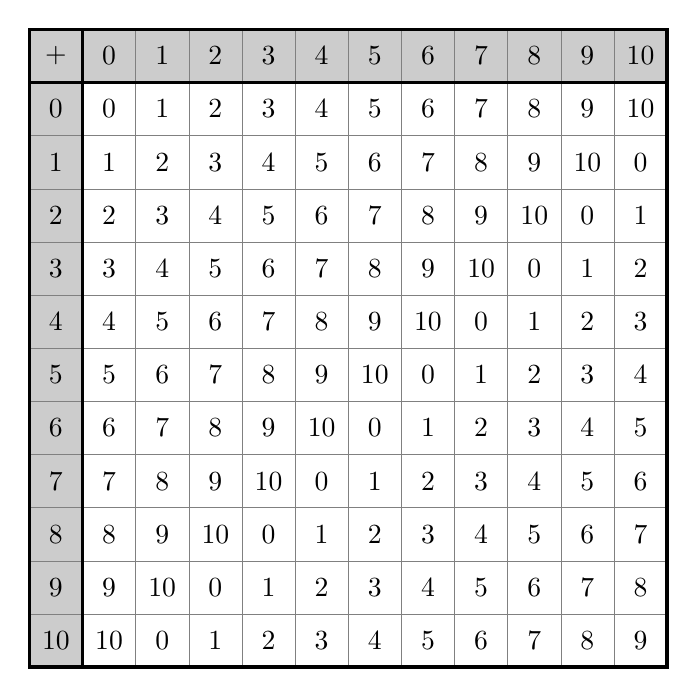
\begin{tikzpicture}[>=latex,thick,scale=0.45]
\fill[color=gray!40] (0,0) rectangle (18,-1.5);
\fill[color=gray!40] (0,0) rectangle (1.5,-18);	
\draw[step = 1.5, gray,very thin] (0,0) grid (18,-18);
\draw[very thick] (0,0) rectangle (18,-18);
\draw[very thick] (0,-1.5) -- (18,-1.5);
\draw[very thick] (1.5,0) -- (1.5,-18);
\node at (0.75,-0.75) {$+$};
\foreach \x in {0,...,10}
	\node at (2.25+\x*1.5,-0.75) {$\x$};
\foreach \y in {0,...,10}
	\node at (0.75,-2.25+\y*-1.5) {$\y$};
% Row 0
\node at ( 2.25,-2.25) {$0$};
\node at ( 3.75,-2.25) {$1$};
\node at ( 5.25,-2.25) {$2$};
\node at ( 6.75,-2.25) {$3$};
\node at ( 8.25,-2.25) {$4$};
\node at ( 9.75,-2.25) {$5$};
\node at (11.25,-2.25) {$6$};
\node at (12.75,-2.25) {$7$};
\node at (14.25,-2.25) {$8$};
\node at (15.75,-2.25) {$9$};
\node at (17.25,-2.25) {$10$};
% Row 1
\node at ( 2.25,-3.75) {$1$};
\node at ( 3.75,-3.75) {$2$};
\node at ( 5.25,-3.75) {$3$};
\node at ( 6.75,-3.75) {$4$};
\node at ( 8.25,-3.75) {$5$};
\node at ( 9.75,-3.75) {$6$};
\node at (11.25,-3.75) {$7$};
\node at (12.75,-3.75) {$8$};
\node at (14.25,-3.75) {$9$};
\node at (15.75,-3.75) {$10$};
\node at (17.25,-3.75) {$0$};
% Row 2
\node at ( 2.25,-5.25) {$2$};
\node at ( 3.75,-5.25) {$3$};
\node at ( 5.25,-5.25) {$4$};
\node at ( 6.75,-5.25) {$5$};
\node at ( 8.25,-5.25) {$6$};
\node at ( 9.75,-5.25) {$7$};
\node at (11.25,-5.25) {$8$};
\node at (12.75,-5.25) {$9$};
\node at (14.25,-5.25) {$10$};
\node at (15.75,-5.25) {$0$};
\node at (17.25,-5.25) {$1$};
% Row 3
\node at ( 2.25,-6.75) {$3$};
\node at ( 3.75,-6.75) {$4$};
\node at ( 5.25,-6.75) {$5$};
\node at ( 6.75,-6.75) {$6$};
\node at ( 8.25,-6.75) {$7$};
\node at ( 9.75,-6.75) {$8$};
\node at (11.25,-6.75) {$9$};
\node at (12.75,-6.75) {$10$};
\node at (14.25,-6.75) {$0$};
\node at (15.75,-6.75) {$1$};
\node at (17.25,-6.75) {$2$};
% Row 4
\node at ( 2.25,-8.25) {$4$};
\node at ( 3.75,-8.25) {$5$};
\node at ( 5.25,-8.25) {$6$};
\node at ( 6.75,-8.25) {$7$};
\node at ( 8.25,-8.25) {$8$};
\node at ( 9.75,-8.25) {$9$};
\node at (11.25,-8.25) {$10$};
\node at (12.75,-8.25) {$0$};
\node at (14.25,-8.25) {$1$};
\node at (15.75,-8.25) {$2$};
\node at (17.25,-8.25) {$3$};
% Row 5
\node at ( 2.25,-9.75) {$5$};
\node at ( 3.75,-9.75) {$6$};
\node at ( 5.25,-9.75) {$7$};
\node at ( 6.75,-9.75) {$8$};
\node at ( 8.25,-9.75) {$9$};
\node at ( 9.75,-9.75) {$10$};
\node at (11.25,-9.75) {$0$};
\node at (12.75,-9.75) {$1$};
\node at (14.25,-9.75) {$2$};
\node at (15.75,-9.75) {$3$};
\node at (17.25,-9.75) {$4$};
% Row 6
\node at ( 2.25,-11.25) {$6$};
\node at ( 3.75,-11.25) {$7$};
\node at ( 5.25,-11.25) {$8$};
\node at ( 6.75,-11.25) {$9$};
\node at ( 8.25,-11.25) {$10$};
\node at ( 9.75,-11.25) {$0$};
\node at (11.25,-11.25) {$1$};
\node at (12.75,-11.25) {$2$};
\node at (14.25,-11.25) {$3$};
\node at (15.75,-11.25) {$4$};
\node at (17.25,-11.25) {$5$};
% Row 7
\node at ( 2.25,-12.75) {$7$};
\node at ( 3.75,-12.75) {$8$};
\node at ( 5.25,-12.75) {$9$};
\node at ( 6.75,-12.75) {$10$};
\node at ( 8.25,-12.75) {$0$};
\node at ( 9.75,-12.75) {$1$};
\node at (11.25,-12.75) {$2$};
\node at (12.75,-12.75) {$3$};
\node at (14.25,-12.75) {$4$};
\node at (15.75,-12.75) {$5$};
\node at (17.25,-12.75) {$6$};
% Row 8
\node at ( 2.25,-14.25) {$8$};
\node at ( 3.75,-14.25) {$9$};
\node at ( 5.25,-14.25) {$10$};
\node at ( 6.75,-14.25) {$0$};
\node at ( 8.25,-14.25) {$1$};
\node at ( 9.75,-14.25) {$2$};
\node at (11.25,-14.25) {$3$};
\node at (12.75,-14.25) {$4$};
\node at (14.25,-14.25) {$5$};
\node at (15.75,-14.25) {$6$};
\node at (17.25,-14.25) {$7$};
% Row 9
\node at ( 2.25,-15.75) {$9$};
\node at ( 3.75,-15.75) {$10$};
\node at ( 5.25,-15.75) {$0$};
\node at ( 6.75,-15.75) {$1$};
\node at ( 8.25,-15.75) {$2$};
\node at ( 9.75,-15.75) {$3$};
\node at (11.25,-15.75) {$4$};
\node at (12.75,-15.75) {$5$};
\node at (14.25,-15.75) {$6$};
\node at (15.75,-15.75) {$7$};
\node at (17.25,-15.75) {$8$};
% Row 10
\node at ( 2.25,-17.25) {$10$};
\node at ( 3.75,-17.25) {$0$};
\node at ( 5.25,-17.25) {$1$};
\node at ( 6.75,-17.25) {$2$};
\node at ( 8.25,-17.25) {$3$};
\node at ( 9.75,-17.25) {$4$};
\node at (11.25,-17.25) {$5$};
\node at (12.75,-17.25) {$6$};
\node at (14.25,-17.25) {$7$};
\node at (15.75,-17.25) {$8$};
\node at (17.25,-17.25) {$9$};
\end{tikzpicture}

\end{center}


\subsection{Multiplikationstabelle
	\label{reedsolomon:subsection:mptab}}
% created by Michael Steiner
%
% Restetabelle von F_11: Multiplikation

% alternatives design
%\begin{figure}
%\begin{center}
%\begin{tabular}{|>{$}c<{$}|>{$}c<{$}>{$}c<{$}>{$}c<{$}>{$}c<{$}>{$}c<{$}>{$}c<{$}>{$}c<{$}>{$}c<{$}>{$}c<{$}>{$}c<{$}>{$}c<{$}|}
%\hline
%\cdot&0&1&2&3&4&5&6&7&8&9&10\\
%\hline
%0&0&0&0&0&0&0&0&0&0&0&0\\
%1&0&1&2&3&4&5&6&7&8&9&10\\
%2&0&2&4&6&8&10&1&3&5&7&9\\
%3&0&3&6&9&1&4&7&10&2&5&8\\
%4&0&4&8&1&5&9&2&6&10&3&7\\
%5&0&5&10&4&9&3&8&2&7&1&6\\
%6&0&6&1&7&2&8&3&9&4&10&5\\
%7&0&7&3&10&6&2&9&5&1&8&4\\
%8&0&8&5&2&10&7&4&1&9&6&3\\
%9&0&9&7&5&3&1&10&8&6&4&2\\
%10&0&10&9&8&7&6&5&4&3&2&1\\
%\hline
%\end{tabular}
%\end{center}
%\end{figure}

\begin{center}
	
	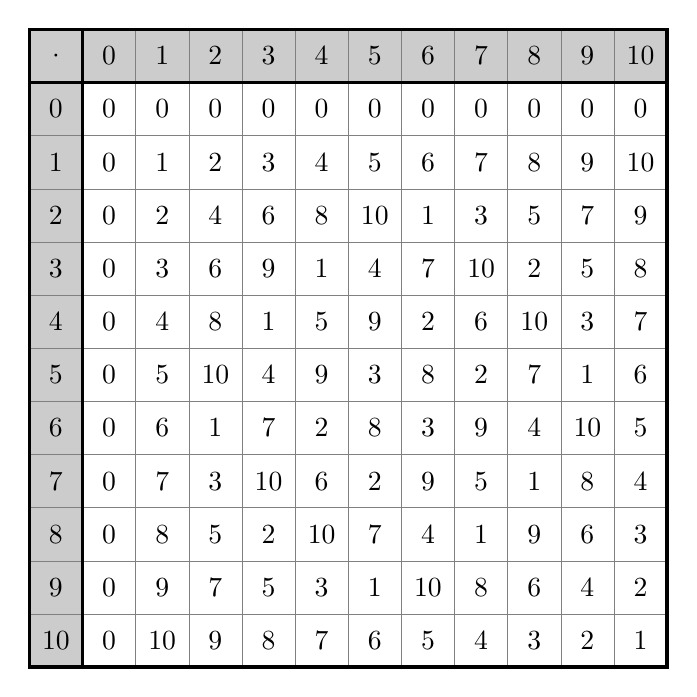
\begin{tikzpicture}[>=latex,thick,scale=0.45]
		\fill[color=gray!40] (0,0) rectangle (18,-1.5);
		\fill[color=gray!40] (0,0) rectangle (1.5,-18);	
		\draw[step = 1.5, gray,very thin] (0,0) grid (18,-18);
		\draw[very thick] (0,0) rectangle (18,-18);
		\draw[very thick] (0,-1.5) -- (18,-1.5);
		\draw[very thick] (1.5,0) -- (1.5,-18);
		\node at (0.75,-0.75) {$\cdot$};
		\foreach \x in {0,...,10}
		\node at (2.25+\x*1.5,-0.75) {$\x$};
		\foreach \y in {0,...,10}
		\node at (0.75,-2.25+\y*-1.5) {$\y$};
		% Row 0
		\node at ( 2.25,-2.25) {$0$};
		\node at ( 3.75,-2.25) {$0$};
		\node at ( 5.25,-2.25) {$0$};
		\node at ( 6.75,-2.25) {$0$};
		\node at ( 8.25,-2.25) {$0$};
		\node at ( 9.75,-2.25) {$0$};
		\node at (11.25,-2.25) {$0$};
		\node at (12.75,-2.25) {$0$};
		\node at (14.25,-2.25) {$0$};
		\node at (15.75,-2.25) {$0$};
		\node at (17.25,-2.25) {$0$};
		% Row 1
		\node at ( 2.25,-3.75) {$0$};
		\node at ( 3.75,-3.75) {$1$};
		\node at ( 5.25,-3.75) {$2$};
		\node at ( 6.75,-3.75) {$3$};
		\node at ( 8.25,-3.75) {$4$};
		\node at ( 9.75,-3.75) {$5$};
		\node at (11.25,-3.75) {$6$};
		\node at (12.75,-3.75) {$7$};
		\node at (14.25,-3.75) {$8$};
		\node at (15.75,-3.75) {$9$};
		\node at (17.25,-3.75) {$10$};
		% Row 2
		\node at ( 2.25,-5.25) {$0$};
		\node at ( 3.75,-5.25) {$2$};
		\node at ( 5.25,-5.25) {$4$};
		\node at ( 6.75,-5.25) {$6$};
		\node at ( 8.25,-5.25) {$8$};
		\node at ( 9.75,-5.25) {$10$};
		\node at (11.25,-5.25) {$1$};
		\node at (12.75,-5.25) {$3$};
		\node at (14.25,-5.25) {$5$};
		\node at (15.75,-5.25) {$7$};
		\node at (17.25,-5.25) {$9$};
		% Row 3
		\node at ( 2.25,-6.75) {$0$};
		\node at ( 3.75,-6.75) {$3$};
		\node at ( 5.25,-6.75) {$6$};
		\node at ( 6.75,-6.75) {$9$};
		\node at ( 8.25,-6.75) {$1$};
		\node at ( 9.75,-6.75) {$4$};
		\node at (11.25,-6.75) {$7$};
		\node at (12.75,-6.75) {$10$};
		\node at (14.25,-6.75) {$2$};
		\node at (15.75,-6.75) {$5$};
		\node at (17.25,-6.75) {$8$};
		% Row 4
		\node at ( 2.25,-8.25) {$0$};
		\node at ( 3.75,-8.25) {$4$};
		\node at ( 5.25,-8.25) {$8$};
		\node at ( 6.75,-8.25) {$1$};
		\node at ( 8.25,-8.25) {$5$};
		\node at ( 9.75,-8.25) {$9$};
		\node at (11.25,-8.25) {$2$};
		\node at (12.75,-8.25) {$6$};
		\node at (14.25,-8.25) {$10$};
		\node at (15.75,-8.25) {$3$};
		\node at (17.25,-8.25) {$7$};
		% Row 5
		\node at ( 2.25,-9.75) {$0$};
		\node at ( 3.75,-9.75) {$5$};
		\node at ( 5.25,-9.75) {$10$};
		\node at ( 6.75,-9.75) {$4$};
		\node at ( 8.25,-9.75) {$9$};
		\node at ( 9.75,-9.75) {$3$};
		\node at (11.25,-9.75) {$8$};
		\node at (12.75,-9.75) {$2$};
		\node at (14.25,-9.75) {$7$};
		\node at (15.75,-9.75) {$1$};
		\node at (17.25,-9.75) {$6$};
		% Row 6
		\node at ( 2.25,-11.25) {$0$};
		\node at ( 3.75,-11.25) {$6$};
		\node at ( 5.25,-11.25) {$1$};
		\node at ( 6.75,-11.25) {$7$};
		\node at ( 8.25,-11.25) {$2$};
		\node at ( 9.75,-11.25) {$8$};
		\node at (11.25,-11.25) {$3$};
		\node at (12.75,-11.25) {$9$};
		\node at (14.25,-11.25) {$4$};
		\node at (15.75,-11.25) {$10$};
		\node at (17.25,-11.25) {$5$};
		% Row 7
		\node at ( 2.25,-12.75) {$0$};
		\node at ( 3.75,-12.75) {$7$};
		\node at ( 5.25,-12.75) {$3$};
		\node at ( 6.75,-12.75) {$10$};
		\node at ( 8.25,-12.75) {$6$};
		\node at ( 9.75,-12.75) {$2$};
		\node at (11.25,-12.75) {$9$};
		\node at (12.75,-12.75) {$5$};
		\node at (14.25,-12.75) {$1$};
		\node at (15.75,-12.75) {$8$};
		\node at (17.25,-12.75) {$4$};
		% Row 8
		\node at ( 2.25,-14.25) {$0$};
		\node at ( 3.75,-14.25) {$8$};
		\node at ( 5.25,-14.25) {$5$};
		\node at ( 6.75,-14.25) {$2$};
		\node at ( 8.25,-14.25) {$10$};
		\node at ( 9.75,-14.25) {$7$};
		\node at (11.25,-14.25) {$4$};
		\node at (12.75,-14.25) {$1$};
		\node at (14.25,-14.25) {$9$};
		\node at (15.75,-14.25) {$6$};
		\node at (17.25,-14.25) {$3$};
		% Row 9
		\node at ( 2.25,-15.75) {$0$};
		\node at ( 3.75,-15.75) {$9$};
		\node at ( 5.25,-15.75) {$7$};
		\node at ( 6.75,-15.75) {$5$};
		\node at ( 8.25,-15.75) {$3$};
		\node at ( 9.75,-15.75) {$1$};
		\node at (11.25,-15.75) {$10$};
		\node at (12.75,-15.75) {$8$};
		\node at (14.25,-15.75) {$6$};
		\node at (15.75,-15.75) {$4$};
		\node at (17.25,-15.75) {$2$};
		% Row 10
		\node at ( 2.25,-17.25) {$0$};
		\node at ( 3.75,-17.25) {$10$};
		\node at ( 5.25,-17.25) {$9$};
		\node at ( 6.75,-17.25) {$8$};
		\node at ( 8.25,-17.25) {$7$};
		\node at ( 9.75,-17.25) {$6$};
		\node at (11.25,-17.25) {$5$};
		\node at (12.75,-17.25) {$4$};
		\node at (14.25,-17.25) {$3$};
		\node at (15.75,-17.25) {$2$};
		\node at (17.25,-17.25) {$1$};
	\end{tikzpicture}
	
\end{center}

\nocite{reedsolomon:weitz}
\nocite{reedsolomon:informationkommunikation}
\nocite{reedsolomon:voyager_programm}
\nocite{reedsolomon:voyager}
\nocite{reedsolomon:cd_wiki}
\nocite{reedsolomon:cd}
\nocite{reedsolomon:qr_wiki}
\nocite{reedsolomon:qr}
%\nocite{reedsolomon:mendezmueller}

\printbibliography[heading=subbibliography]
\end{refsection}
